\documentclass[12pt, twoside]{fithesis2}

% ===== LOADING PACKAGES =====
% language settings
\usepackage[english]{babel}
% enabling new fonts support (nicer)
\usepackage{lmodern}
% setting input encoding
\usepackage[utf8]{inputenc}
% setting output encoding
\usepackage[T1]{fontenc}
% fithesis2 requires csquotes
\usepackage{csquotes}
% set page margins
\usepackage[top=3.0cm, bottom=3.5cm, left=2.9cm, right=1.9cm]{geometry}
% package to make bullet list nicer
\usepackage{enumitem}
% math symbols and environments
\usepackage{mathtools}
\usepackage{amsmath}
\usepackage{amssymb}
% packages for complex tables
\usepackage{tabularx}
% package for defining new floating environments
\usepackage{float}
\usepackage[labelfont=]{caption}
% package for drawing
\usepackage{tikz}
\usetikzlibrary{shapes,positioning,fit,plotmarks}
% code listings
\usepackage{listings}

% space between paragraphs
\setlength{\parskip}{0.6em plus0.2em minus0.2em} % zkraceni vzdalenosti mezi odstavci

% bibliography management
\usepackage[backend=biber, 		% use biber as backend instead of BiBTeX
        %dashed=false                    % when there is an author twice, still write his/her name
	bibstyle=ieee-alphabetic, 	% bibliography style: IEEE with alphabetic citations
	citestyle=alphabetic, 		% citation style
	url=true, 			% display urls in bibliography
	hyperref=auto,			% detect hyperref and create links
	%block=ragged, 			% format bibliography into blocks, ragged on right
]{biblatex}
\addbibresource{thesis.bib}
% break long urls
\setcounter{biburllcpenalty}{7000}
\setcounter{biburlucpenalty}{8000}

% setting custom colors for links
\usepackage{xcolor}
\definecolor{theme-red}{rgb}{0.62,0.01,0.05}
\definecolor{dark-red}{rgb}{0.6,0.15,0.15}
\definecolor{dark-green}{rgb}{0.15,0.4,0.15}
\definecolor{medium-blue}{rgb}{0,0,0.5}
\definecolor{light-gray}{rgb}{0.93,0.93,0.93}
% generating hyperlinks in document
\usepackage{url}
\usepackage[plainpages=false, 	    % get the page numbering correctly
            pdfpagelabels, 	    % write arabic labels to all pages
            unicode,	 	    % allow unicode characters in links
            colorlinks=true, 	    % use colored links instead of boxed (pc version)
            %hidelinks, 		    % hide links (print version)
            %linkcolor={dark-red},
            %citecolor={dark-green},
            %urlcolor={medium-blue}
            linkcolor={theme-red},
            citecolor={theme-red},
            urlcolor={theme-red}
			]{hyperref}

% ===== FI THESIS SETTINGS =====

\thesistitle{Automatic Question Generation\\and Adaptive Practice}
\thesissubtitle{Bachelor thesis}
\thesisstudent{Tomáš Effenberger}
\thesiswoman{false}
\thesisfaculty{fi}
\thesisyear{spring 2015}
\thesisadvisor{RNDr.\ Jan Rygl}
\thesislang{en}

% ===== LATEX DOCUMENT SETTINGS =====

% only put chapters and sections into the TOC
\setcounter{tocdepth}{2}   % nefunguje (podle navodu by melo fungovat s 1, ale neni tomu tak)


% adjusting hyphenation penalties
%\tolerance=10000
%\hyphenpenalty=500

% hyphenations settings
\hyphenation{DBpedia}

% renew command for shorter and nicer underscore
\renewcommand{\_}{\leavevmode \kern0.07em\vbox{\hrule width0.4em}}


% ===== COMMANDS =====

%--------------------------------------------------------------------
% define square symbol
%--------------------------------------------------------------------
\newcommand{\squarebullet}{\textcolor{black}{\raisebox{0.15em}{\rule{4pt}{4pt}}}}
\newcommand{\emptysquarebullet}{\textcolor{black}{\raisebox{0.10em}{\tiny$\square$}}}

%--------------------------------------------------------------------
% define new itemize environment with squares and smaller spaces
%--------------------------------------------------------------------
\newenvironment{myItemize}{
  \begin{itemize}[leftmargin=2em,rightmargin=1em,itemsep=\parskip ,parsep=0em,topsep=0em,partopsep=0em]
  \renewcommand{\labelitemi}{\squarebullet}
  %\renewcommand{\labelitemii}{$\diamond$}
  %\renewcommand{\labelitemii}{\emptysquarebullet}
  \renewcommand{\labelitemii}{\textbullet}
}{
  \end{itemize}
}

\newenvironment{myEnumerate}{
  \begin{enumerate}[leftmargin=2em,rightmargin=1em,itemsep=\parskip ,parsep=0em,topsep=0em,partopsep=0em]
}{
  \end{enumerate}
}

%--------------------------------------------------------------------
% define new environment for Python code
%--------------------------------------------------------------------

%\lstset{%
%  language=SQL,%
%  morekeywords={PREFIX,LIMIT},%
%  basicstyle=\small\ttfamily,
%  frame=single%
%}

\lstnewenvironment{code}{%
  \lstset{backgroundcolor=\color{light-gray},
  frame=lines,
  %framerule=1pt,
  rulecolor=\color{black},
  basicstyle=\ttfamily,
  columns=fullflexible,
  showspaces=false,
  showstringspaces=false,
  escapeinside={<*}{*>},
  belowskip=0.2em,
  morekeywords={Pattern,Question,Answer,Filter,Relation}
  }}{}

% define command for splitting listings into "from" and "to" part
\newcommand{\arrowlinesplit}{%
  \noindent\makebox[\linewidth]{\raisebox{0.15em}{\rule{0.478\textwidth}{0.5pt}}%
  ~$\downarrow$~%
  \noindent\raisebox{0.15em}{\rule{0.478\textwidth}{0.5pt}}}%
}

%--------------------------------------------------------------------
% exercise environment
%--------------------------------------------------------------------
\newcounter{choice}
\renewcommand\thechoice{\Alph{choice}}
\newcommand\choicelabel{\thechoice.}

\newenvironment{choices}%
  {\vspace{0.8em}\list{\choicelabel}%
     {\usecounter{choice}\def\makelabel##1{\hss\llap{##1}}%
       \settowidth{\leftmargin}{W.\hskip\labelsep\hskip 0.01em}%
       \def\choice{%
         \item
       } % choice
       \labelwidth\leftmargin\advance\labelwidth-\labelsep
       \topsep=0pt
       \partopsep=0pt
     }%
  }%
  {\vspace{-0.7em}\endlist}

%\setlength{\abovecaptionskip}{25pt plus 3pt minus 2pt}
\floatstyle{boxed}
\newfloat{exercise}{thp}{exrcs}[chapter]
\floatname{exercise}{Exercise}

\newenvironment{question}
{
  \begin{center}
  \vspace{-0.5em}
  \begin{tabular}{p{0.9\textwidth}}
  %\vskip 0.05em
}
{
  \\
  \end{tabular}
  \vspace{-1em}
  \end{center}
}

% gap in the sentence (bottom line)
\newcommand{\sentenceGap}{\rule{1.5cm}{0.4pt}~}

%--------------------------------------------------------------------
% transformation examples
%--------------------------------------------------------------------
\newcommand{\transformationExample}[3]{%
\vspace{-0.5em}
\noindent %
\begin{tabularx}{\linewidth}{@{} l X @{}}
Sentence: & \emph{#1}\\
Question: & \emph{#2}\\
Answer:   & \emph{#3}\\
  \hline
\end{tabularx}
%\vspace{0.2em}
}

%--------------------------------------------------------------------

% ===== DATA =====
%\begin{filecontents}{knowledge-estimate.data}
%0 0
%1 0.29
%2 -0.05
%3 0.35
%4 0.76
%5 1.25
%6 1.31
%7 1.29
%8 0.94
%9 1.19
%\end{filecontents}


% ===== BEGIN DOCUMENT =====
\begin{document}

\FrontMatter
\ThesisTitlePage

\begin{ThesisDeclaration}
\DeclarationText
\AdvisorName
\end{ThesisDeclaration}

\begin{ThesisThanks}
  I would like to thank Jan Rygl
  for his guidance and support, and for his wisdom and infinite kindness.
  I would also like to thank members of the Natural Language Processing Centre
  and Adaptive Learning group for fruitful discussions,
  and all my friends who helped me to test the developed application
  and came up with a lot of great suggestions for future development.
\end{ThesisThanks}

\begin{ThesisAbstract}
When studying, it is more efficient not just to read about the topic, but also to practice the knowledge, e.g. by answering some multiple choice questions.
Today, there is a huge amount of information to study (consider Wikipedia) and it is not possible to create a set of questions for all topics manually.
However, we can generate questions automatically, using techniques of artificial intelligence and natural language processing.
This thesis explores the state-of-the-art approaches to question generation and describes their advantages and disadvantages.
The thesis also suggests a design of the general framework for practicing knowledge from articles.
The framework is implemented and publicly accessible through a web interface.
\end{ThesisAbstract}

\begin{ThesisKeyWords}
% TODO: profiltrovat na ty opravdu relevantni
question generation, adaptive practice,
learning,
multiple choice questions,
knowledge representation, knowledge extraction
%artificial intelligence, natural language processing,
\end{ThesisKeyWords}

\MainMatter
\tableofcontents

% ===========================  CHAPTER ===========================
\chapter{Introduction}
\label{chap:intro}

Repeated reading of the text is an inefficient method of learning,
while answering to the related questions leads to better understanding and remembering \cite{edu-improve}.
Creating questions for a given topic is a time-consuming task
and it is not possible to create a set of questions for each topic manually.
However, we can generate questions automatically, using techniques of artificial intelligence and natural language processing.
This thesis explores the state-of-the-art approaches to question generation and describes their advantages and disadvantages.

In spite of an active research in the field of question generation
(boosted by the question generation shared task and evaluation challenge in 2009 \cite{shared-task2009}),
there is still no publicly available web application to solve this task (as of April 2015).
An online application for question generation would be invaluable.
Typical example of usage is to make self-studying more efficient by answering a few generated questions after reading an article to verify and consolidate the knowledge acquired from the text.

That is why I have implemented the \textit{Smartoo, Smart Artificially Intelligent Tutor}, modular and extensible framework for question generation and adaptive practice
of knowledge from the \emph{Wikipedia}%
\footnote{\url{http://en.wikipedia.org/}}
articles.
The Smartoo framework is licensed under the GNU General Public License, version 2.
The source code is available from its \textit{GitHub repository}%
\footnote{\url{http://github.com/effa/smartoo}}.
The prototype behavior has been deployed and is publicly available%
\footnote{\url{http://smartoo.thran.cz}}.

The thesis text is structured as follows.
In \autoref{chap:knowledge}, I discuss the knowledge extraction from the text,
which might precede the actual question generation.
The question generation, together with the issue of ranking and filtering of the generated questions are the subject of \autoref{chap:exercises}.
In \autoref{chap:practice}, I talk about some common strategies for the adaptive practice, which is essential for a good learning experience.
In \autoref{chap:smartoo}, I describe the implemented Smartoo framework
and \autoref{chap:evaluation} contains details about its deployment and evaluation.
Finally, in \autoref{chap:future}, I present planned future development of the Smartoo framework.




% ===========================  CHAPTER ===========================
\chapter{Knowledge Extraction and Representation}
\label{chap:knowledge}

Instead of creating exercises directly from the text in natural language (unstructured data),
one can at first attempt to extract the meaning from the text,
i.e. convert the text into the structured data.
This process is called \textit{information extraction} \cite[][262]{nlp-python}.
Information extraction has several subtasks, the two most relevant for us are:
\begin{myItemize}
  \item \textit{named entity recognition} -- extraction of terms (e.g. \textit{Abraham Lincoln}) and numeric expressions (e.g. \emph{12 February 1809}) (more detailed definition is in \autoref{sec:terms-extraction}),
  \item \textit{relation extraction} -- extraction of relations between the discovered named entities,
    for example \emph{birhDate(Abraham Lincoln, 12 February 1809)}
    (\autoref{sec:relations-extraction}).
\end{myItemize}

One way to create exercises is to first perform the relation extraction and then create the exercises from built structured knowledge representation. Another approach is to generate exercises from text with discovered named entities. We will take a closer look at both of these approaches in \autoref{chap:exercises}.

Before the discussion of the named entity recognition and relation extraction,
I will talk about how to represent the extracted knowledge.
Knowledge can be represented in many ways,
such as using first order logic, semantic nets or frames \cite{knowledge-representation}.
In the following section, I will describe \emph{RDF graphs},
since we will use this knowledge representation in the other chapters.

\begin{figure}[h]
  \centering
  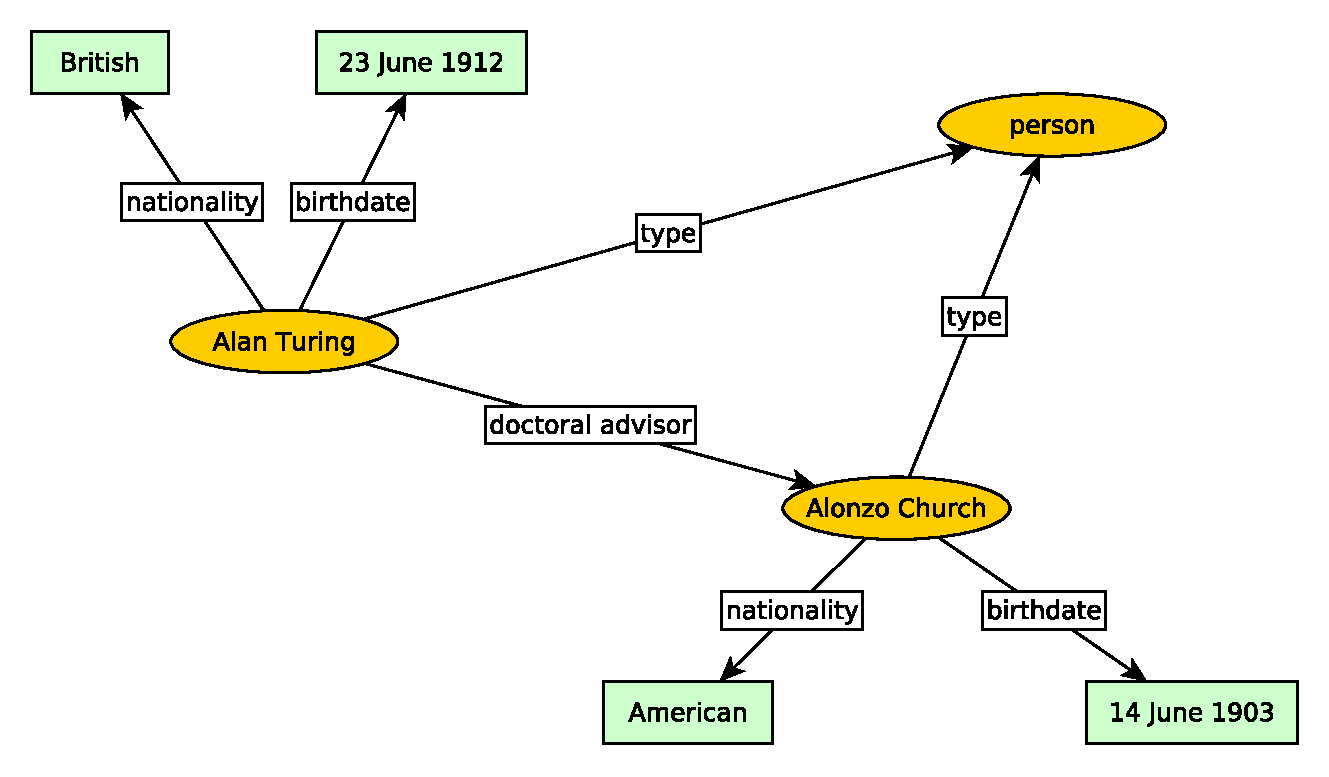
\includegraphics[width=\textwidth]{images/rdf-graph.pdf}
  \caption{Simple RDF graph}
  \label{fig:simple-rdf-graph}
\end{figure}

% ---------------------------  SECTION  ---------------------------
\section{RDF Graph}
\label{sec:rdf-graph}

%One common way is to represent knowledge as a graph (\textit{knowledge graph}), where vertices are named entities
%and edges indicate relations between the entities.

RDF%
\footnote{\textit{Resource Description Framework}.
See \url{http://www.w3.org/standards/techs/rdf} for RDF standards.}
graph is a collection of subject-predicate-object triples \parencite[][63]{semantic-web}.
Each triple is called a \textit{fact}.
Simple example of a few facts about Alan Turing and Alonzo Church follows:
\begin{code}
Alan Turing - type - person
Alan Turing - birthdate - 23 June 1912
Alan Turing - nationality - British
Alan Turing - doctoral advisor - Alonzo Church
Alonzo Church - type - person
Alonzo Church - nationality - American
Alonzo Church - birthdate - 14 June 1903
\end{code}
\noindent
\autoref{fig:simple-rdf-graph} shows how can be this collection of facts thought of as a directed graph.
Vertices corresponds to subjects and objects. Each fact maps to one edge, with direction from the subject to the object and with edge value given by the predicate.

To avoid possible ambiguity (e.g. between two people who have both name \textit{Alan Turing})
unique URIs%
\footnote{\emph{Uniform Resource Identifier}. See RFC 3986 (\url{https://tools.ietf.org/html/rfc3986}) for details.}
are used to represent subject, objects and predicates.
URI consists of a prefix and a name:%
\footnote{Different entities can have same name, for example \texttt{http://dbpedia.org/resource/Apple} and \texttt{http://smartoo.com/term/Apple}.}
\begin{center}
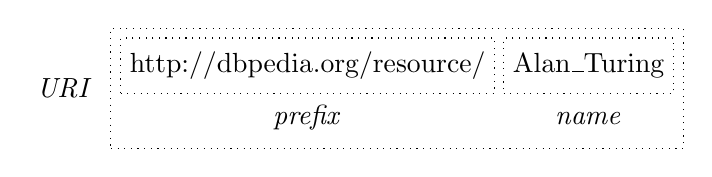
\begin{tikzpicture}[scale=1]
    \tikzstyle{part} = [draw,rectangle,dotted,fill=none,minimum height=0.7cm]
    %\tikzstyle{caption} = [plain,draw=none,fill=none]
    \tikzstyle{mylabel} = [text width=5em, text centered]
    \node[part] (prefix) at (0,0) {http://dbpedia.org/resource/};
    \node[part] (name) [right = 1mm of prefix] {Alan\_Turing};
    \node[mylabel] (label1) [below = 0.2mm of prefix] {\textit{prefix}};
    \node[mylabel] (label2) [below = 1.2mm of name] {\textit{name}};
    \node[part,fit=(prefix) (name) (label1) (label2)] (uri) {};
    \node (label3) [left = 1mm of uri] {\textit{URI}};
\end{tikzpicture}
\end{center}
\noindent
Objects can be either URIs or literals, such as numbers, strings or dates (e.g. \emph{1912-06-23}).
Simple example with prefixes (part of the graph above) follows:
\begin{code}
<http://dbpedia.org/resource/Alan_Turing>
    <http://www.w3.org/1999/02/22-rdf-syntax-ns#type>
    <http://xmlns.com/foaf/0.1/Person> .
<http://dbpedia.org/resource/Alan_Turing>
    <http://dbpedia.org/ontology/birthDate>
    1912-06-23+02:00
<http://dbpedia.org/resource/Alan_Turing>
   <http://dbpedia.org/property/nationality>
   "British"@en
\end{code}

The used format is called \textit{N-Triples} \cite[][68]{semantic-web}.
There are several others serializations of RDF graph, such as \textit{RDF/XML}
\cite[][73]{semantic-web}
or \emph{Turtle (Terse RDF Triple Language)},
which makes the serialization shorter by grouping facts by subjects (possibly also predicates) and by using shortcuts for prefixes. The same graph as above would look like this in the Turtle syntax:

\begin{code}
@prefix rsrc: <http://dbpedia.org/resource/>
@prefix rdf: <http://www.w3.org/1999/02/22-rdf-syntax-ns#>
@prefix dbpedia-owl: <http://dbpedia.org/ontology/>
@prefix dbprop: <http://dbpedia.org/property/>
@prefix foaf: <http://xmlns.com/foaf/0.1/>

rsrc:Alan_Turing
  rdf:type foaf:person ;
  dbpedia-owl:birthDate 1912-06-23+02:00 ;
  dbprop:nationality "British"@en .
\end{code}

RDF graph is great for a representation of simple facts (\emph{declarative knowledge}),
but it is useful to know about its limitations.
In particular, RDF graphs are not designed to capture \textit{procedural knowledge}, such as mathematical problem solving.

%[MaybeTODO: takze nemuzeme pak testovat higher order thinking skills... citace k tomu higher order thinking skills, napr. Bloom's taxonomy]


% ---------------------------  SECTION  ---------------------------
\section{SPARQL}
\label{sec:sparql}

\textit{SPARQL}%
\footnote{The name of this query language is a recursive acronym of \textit{SPARQL Protocol and RDF Query Language}.}
is a query language for convenient querying of RDF graphs \parencite[][84]{semantic-web}.
The most common query is the \textit{select query} which resembles SQL select query and has the following main parts:
\begin{myItemize}
  \item \textbf{prefix} -- definition of prefixes and associated shortcuts,
  \item \textbf{from} -- dataset (RDF graph) on which to run the query,
  \item \textbf{select} -- which information to return,
  \item \textbf{where} -- condition on returned data,
  \item \textbf{order by} -- ordering of results.
\end{myItemize}
Variables are prefixed by a ``?''. As an example, have a look at the following SPARQL query, which would return the birthdate and birthplace of Alan Turing:
\begin{code}
PREFIX rsrc: <http://dbpedia.org/resource/>
PREFIX owl: <http://dbpedia.org/ontology/>
SELECT ?date ?place
WHERE {
  rsrc:Alan_Turing owl:birthDate ?date ;
                     owl:birthPlace ?place .
}
\end{code}

More examples of SPARQL queries can be found in the section about creating exercises from knowledge graphs
(\autoref{sec:exercises-from-knowledge-graph}).

%% ---------------------------  SECTION  ---------------------------
%\section{Ontology}
%\label{sec:ontology}

%TODO: ontologie - co to je, k cemu to je
%- v dalsi kapitole (odkaz) bude rozebrano, jak generovat otazky s vyuzitim ontologii

%O co jde: ontologií se rozumí popis vlastností, tříd a jejich hierarchie
%(mezi tridou a podtridou je "is-a" relationship)


% ---------------------------  SECTION  ---------------------------
\section{Named Entity Recognition}
\label{sec:terms-extraction}
\textit{Named entities}
are ``information units like names, including person, organization and location names, and numeric expressions including time, date, money and percent expressions'' \autocite{named-entity-recognition}.
Sometimes, I will specifically refer to \textit{terms}, which are named entities other than numeric expressions.
As an example, \textit{Abraham Lincoln} is a term, while \textit{21 March 2015} is a numeric expression.
%(and both are named entities).
The aim of the \textit{named entity recognition} is to discover all named entities in a given text and label them with their types. Common types of named entities are organization, person, location, date, time, money, percent, facility and geo-political entity \cite[][281]{nlp-python}. There are several approaches to the task of named entity recognition:
\begin{myItemize}
\item \textbf{Regular expressions}\\
  Regular expressions are especially good for numeric expressions as they typical follow reasonably simple rules.
  As an example, consider the following regular expression (in Python dialect%
  \footnote{\url{https://docs.python.org/2/library/re.html}})
  to capture dates such as \emph{21 March 2015}:
\begin{code}
(?P<date>
    # day (one or two digits followed by a space)
    \d{1,2} \s
    # month (followed by a space)
    (?: January | February | March | April | May | June | July |
         August | September | October | November | December) \s
    # year (four digits)
    \d{4}
)
\end{code}


\item \textbf{List of terms}\\
  A simple way to find if some word or phrase is a named entity is to try to look it up in a list of named entities. There are for example publicly available \textit{gazetteers} -- lists of well-known geographical locations. However, this method is quite limited as it is impossible to have complete lists of all named entities.
(In particular there is infinitely many numeric expressions.)
Another problem is ambiguity of words, e.g. \textit{Reading} is a town in the United Kingdom, but not in the sentence \textit{Reading is important for everyone's personal development.}
  There is one exception when this method works great -- if there is a known list of terms which can appear in the text. For example for each article on the Wikipedia the list of terms can be built from internal links which appear in the article. I use this fact in the Smartoo (\autoref{sec:articles-parsing}).

\item \textbf{Frequency counting}\\
  After identifying nouns and noun phrases in the text, their relative frequencies are calculated and these which exceed a given threshold are considered as terms.
  This method is used by Mitkov \cite{question-gen-mitkov}. It works reasonable well for terms recognition, but it can't discover numeric expressions.
This method can unfortunately also label as terms common names which are frequently used.
A solution to this problem is to apply \textit{tf-idf weighting} which normalizes term frequency in the document by its frequency in all documents (or in common texts) \cite[][118]{information-retrieval}.

\item \textbf{Machine learning}\\
  The most difficult, but also the most powerful method is to use a machine learning-based classifier.
  Traditionally, supervised learning dominated in this field,
  but as it requires a lot of annotated sentences,
  novel approaches using semi-supervised or even unsupervised learning are developed
  \cite{named-entity-recognition}.
  Semi-supervised learning is often based on the method of \emph{bootstrapping} -- a few named entities of each type are given to the system, the system finds them in a large unannotated corpus a uses their context to find other similar named entities, and the whole process is repeated many times with increasing number of discovered named entities and contexts.
\end{myItemize}
Often, several of these approaches are combined, e.g. \textit{The Mentor} (question generation tool) uses regular expressions, gazetteers and a machine learning recognizer \cite{mentor}).


% ---------------------------  SECTION  ---------------------------
\section{Relation Extraction}
\label{sec:relations-extraction}

Having discovered named entities, we can extract relations between them.
For simplicity, we restrict our attention to binary relations,
i.e. relations of the form \emph{relation(a, b)},
%(where \emph{a} and \emph{b} are named entities),
for example \emph{birhDate(Abraham Lincoln, 12 February 1809)}.
Relations of this form can be directly stored in a RDF graph as a subject-predicate-object triple
\emph{(a, relation, b)}.

One way to tackle this task is to consider each pair of named entities which are in the same sentence and decide in which relation they are (or that they are not in any relation) according to words between them \cite[][284]{nlp-python}.
As an example, consider the following pattern for \emph{birthDate} relation between a person and a date:
\begin{code}
Pattern: PERSON was born .* (in | on) DATE
<*\arrowlinesplit*>
Relation: birthDate(PERSON, DATE)
\end{code}
This pattern covers all of the three following cases:
\begin{myItemize}
  \item \emph{Abraham Lincoln was born in 1809.}
  \item \emph{Abraham Lincoln was born on 12 February, 1809.}
  \item \emph{Abraham Lincoln was born in Hodgenville, Kentucky, on 12 February, 1809.}
\end{myItemize}

%- vzory jsou zadany rucne, nebo muzeme zkusit se je naucit pomoci strojoveho uceni from a training corpus.

Relation extraction can be also formulated as a classification problem:
given a sentence with two named entities \emph{a} and \emph{b} and a particular relation type $r$,
decide, if \emph{a} and \emph{b} are in the relation $r$ \cite{rel-extract-review}.
If there are enough positive and negative labeled examples for each relation of our interest,
supervised learning can be used, with features such as
types of the named entities, words between them,
number of words between them, path between them in a syntactic tree of the sentence, etc.
\cite{rel-extract-feature-based}.
As an alternative to the feature based methods, which take a vector of extracted features as an input,
\emph{kernel methods} are sometimes used, which take the full representation of the sentence, possibly with some structural information as an input \cite{rel-extract-kernel}.
% structural information = oznacene named entities a treba shallow parsed sentence
As creating a large labeled training sets is usually expensive, semi-supervised learning became popular as well,using the bootstrapping method (which was described in the previous section) \cite{rel-extract-bootstrapping}.

The mentioned approaches work only if the relation types are known in advance,
so that patterns are written or a classifier is trained for each of the relation.
For unrestricted domain,
we can try to find the relation type in the sentence itself.
For example, from a simple sentences with a subject, a verb and an object,
relation \emph{verb(subject, object)} may be extracted \cite{triples-acquisition}.
However, sentences are often quite complex, so this method requires to preprocess and simplify the text in order to work.

% ---------------------------  SECTION  ---------------------------
\section{Knowledge Bases}
\label{sec:knowledge-bases}

There are several huge publicly available knowledge bases,
which try to capture as many facts about the world as possible.
Examples of popular knowledge bases are
\textit{DBpedia} \cite{dbpedia}
%\footnote{\url{http://dbpedia.org/}}
and \textit{Freebase} \cite{freebase}.
%\footnote{\url{https://www.freebase.com/}}
Knowledge bases are used for many task in natural language processing,
such as
%named entity recognition
named entity disambiguation \cite{dbpedia-spotlight},
semantic search and question answering \cite{watson}.
%-- several knowledge bases (including DBpedia) were used in \emph{DeepQA project} to create \emph{IBM Watson} computer, which won the \emph{Jeopardy!} quiz game against two human champions in 2011 \cite{watson}.
And we can make use of the information in these knowledge bases to create better exercises as well,
for example to select appropriate incorrect alternatives in multiple choice questions
(see \autoref{sec:distractors}).

DBpedia was built by extracting structured information from Wikipedia,
such as titles, links between articles, external links, information from infoboxes and categories.
Facts are stored in the form of an RDF graph.
Whole knowledge base can be be downloaded%
\footnote{\url{http://wiki.dbpedia.org/Downloads}}, %
%data available under \emph{Creative Commons Attribution-ShareAlike License}
%and \emph{GNU Free Documentation License}}.
and it is also possible to use public \textit{DBpedia SPARQL endpoint}.%
\footnote{\url{http://dbpedia.org/sparql}}

\emph{DBpedia Version 2014}
%\footnote{\url{http://wiki.dbpedia.org/Downloads2014}}
contains approximately 580 million facts (RDF triples) retrieved from the English Wikipedia,
describing 4.5 million of things \cite{dbpedia}.
Ontology%
\footnote{Ontology is a description of properties, classes and their hierarchy.}
of DBpedia includes more than 650 classes and 2700 properties.
In \autoref{fig:dbpedia-classes}, a fraction of DBpedia class hierarchy is shown.
\begin{figure}[h]
  \centering
  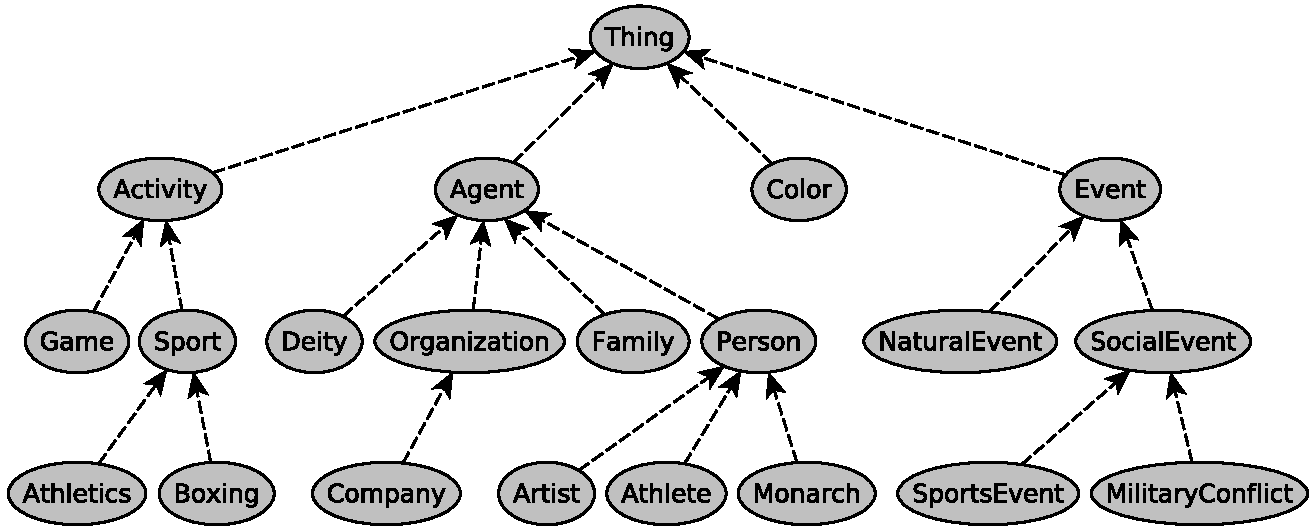
\includegraphics[width=\textwidth]{images/dbpedia-classes.pdf}
  \caption{A fraction of DBpedia class hierarchy. Edges represent subclass relationship.}
  \label{fig:dbpedia-classes}
\end{figure}


% =========================== CHAPTER ===========================
\chapter{Question Generation}
\label{chap:exercises}

The first question generation tool was introduced as early as in the 1970s \cite{questions-wolfe}
and up to now (2015), several approaches to the task of question generation were proposed.
Every system uses different methods and although usually the authors perform some kind of evaluation (e.g. by two people ranking generated questions as good or bad), it is not possible to say which approach is the best as the systems work in different settings, use different source texts from which the questions are generated, create different question types, have different target groups and use different evaluation metrics.
For example some systems try to assess vocabulary \cite{question-gen-vocabulary}
or reading comprehension \cite{question-overgenerating-rating},
some focus on factual texts \cite{question-gen-heilman}
and sometimes authors use for evaluation only a single textbook or a topic, such as linguistics \cite{question-gen-mitkov} or biology \cite{question-gen-textbooks}.

Based on reported performances of the systems, it can be concluded that question generation is still open problem in the natural language processing and there is plenty of room for improvements or even completely new ideas.
Some systems proved to be usable in the offline mode, in which a teacher submits a text to the system,
the system outputs a list of questions and it is assumed that the teacher will filter them and make some corrections in the generated questions. Ideally, there is only a few questions that need to be discarded or corrected and so this semi-automated process of creating questions is faster than creating them fully manually
\cite{question-gen-mitkov}.

Although the chapter is called \textit{question generation},
it is possible to create more complex exercises as well.
Broader range of exercises is especially useful if we want not only to assess one's knowledge, but rather to deepen his or her remembering and understanding of the text.
Generally, people are more likely to remember things that entertain them.
However, complex exercises are more difficult to implement and evaluate,
so usually only questions are generated, most often multiple choice questions.
\textit{Multiple choice questions} consist of a question text (called \textit{stem})
and a few (e.g. four) \textit{choices}, from which one is the \textit{correct answer}
and the rest are incorrect alternatives (called \textit{distractors}).
Special type of multiple choice question is \textit{fill-in-the-blank multiple choice question},
in which the stem is a sentence with a blank space which should be filled with the correct answer.

Although the approaches to the question generation are diverse,
some common tasks can be identified throughout the systems.
The general workflow has the following 5 steps, although some of them may be missing in some systems:
\begin{myEnumerate}
\item First, text of the article is pre-processed.
Pre-processing can range from mere sentence filtering,
to text rephrasing, and even to knowledge extraction from the text and building a knowledge graph
(\autoref{sec:text-pre-processing}).

\item The text is then scanned for the patterns which define transformations from sentences to a question-answer pairs.
  Every time a pattern is matched, a new question and the corresponding answer are generated
  (\autoref{sec:sentence-transformations}).
  If a knowledge graph is used instead of text, the procedure is similar, except that now we have transformations from facts in the knowledge graph. The main advantage is that we can make use of relationships between subjects in the graph and thus create questions which span more then one sentence in the original article
  (\autoref{sec:exercises-from-knowledge-graph}).

\item In case of multiple choice questions, suitable distractors (incorrect alternatives) are selected
(\autoref{sec:distractors}).

\item In the previous steps, questions are usually overgenerated, so it is important to filter them at the end
  (\autoref{sec:questions-ranking-filtering}).
  Instead of direct filtering, we can rank the questions and either select some predefined number of questions with the highest rank
  or employ adaptive practice.
In adaptive practice, decisions about which question is next presented to the student
are not made in advance, but during the practice itself,
based on already answered questions and success of the student.
(Adaptive practice is discussed in detail in chapter \autoref{chap:practice}.)
\end{myEnumerate}

% ---------------------------  SECTION  ---------------------------
\section{Text Pre-processing}
\label{sec:text-pre-processing}

Usually, the text of the document is pre-processed before it is used for question generation.
Pre-processing may
add useful information to the text (e.g. part-of-the-speech tags, semantic role labels),
remove useless sentences (e.g. sentences without information about the topic),
modify (rephrase) sentences or even create different (more machine readable) representation of the knowledge contained in the article, such as a knowledge graph.
%Pre-processing can be conservative or non-conservative.
%I call pre-processing \textit{conservative}, if the output of the pre-processing is still some text,
%while the \textit{non-conservative} pre-processing leads to different (more machine readable) representation of the knowledge.
%Furthermore, we can distinguish between \textit{strongly conservative pre-processing},
%which does not add anything to the text, just filters some of the original sentences, and \textit{weakly conservative pre-processing}, which modifies the actual text of the sentences.
\begin{myItemize}
  \item \textbf{Parsing and labelling}\\
    The text is split into sentences and each sentence is tokenized (\emph{tokens} are words and punctuation).
    Afterwards, each sentence might be \emph{syntactically parsed} (its syntax tree is built)
    or at least \textit{shallow-parsed} (each token is assigned a part-of-the-speech tag).
    Named entities recognition or even semantic role labelling might be performed
    (see \autoref{sec:sentence-transformations} for details).

  \item \textbf{Filtering}\\
    The goal of the filtering is to discard sentences which are not relevant to the article or has not enough context to generate a question from them.
    Typical example of a sentence without sufficient context are \emph{anaphoric references},
    i.e. referring back to something mentioned earlier in the text.
    For example, in the sentence \emph{He was the 16th President of the United States.},
    the word \emph{he} refers to \emph{Abraham Lincoln}.
  Some possible heuristics to detect which sentences cannot be used to generate good questions \cite{questions-wolfe} are:
  \begin{itemize}
  \item sentence is too long (e.g. more than 35 words),
  \item contains demonstrative word (such as \emph{this} and \emph{that}),
  \item starts with a verb.
  \end{itemize}

  Instead of heuristics, we can use a more sophisticated machine learning-based classifier to select only the sentences which are informative, relevant to the topic and have enough context so that questions can generated from them. This approach was tested by Agarwal \cite{question-gen-textbooks}.
Some of the features used in his classifier were:
  \begin{itemize}
  \item the number of words in the sentence,
  \item the number of nouns,
  \item the number of words from the headline,
  \item contains abbreviation? (binary feature),
  \item contains superlativum? (binary feature).
  \end{itemize}

%TODO: poznamka o \textit{content selection}, ze to nemusi byt vzdy skoro vsechno, ale treba jen 1 nebo 6 otazek na odstavec (1 \cite{questions-wolfe}, 6 \cite{question-gen-mannem}) nebo muzeme rovnou hledat pomoci klasifikatoru pouze nejrelevatnejsi vety (Agarwal \cite{question-gen-textbooks}). Ale vetsinovy pristup je otazky nadgenerovat a filterovat pozdeji.

  \item \textbf{Text rephrasing}\\
    Ideal text for question generation would contain exactly one fact in one sentence,
    but in reality most of the sentences are either too complex (consisting of many clauses)
    or they lack important context (e.g. due to using pronouns).
    We might want to transform (rephrase) the original text into simple factual sentences
    \cite{question-gen-heilman,question-improv-foster},
    for example split complex sentences into simple ones,
    remove unimportant information (such as content of brackets)
    and resolve anaphoras.

    %Konkretne: \cite{question-gen-heilman}: rozdeleni slozene vety na jednoduche, vynechani nedulezitych extra informaci (napr. zavorky nebo non-restrictive appositives (Jeffereson, the third president of the United States, ...), pronoun resolution (difficult...), ale aspon uvest priklad

    %TODO: o tom jak rozdelit complex sentences na seriii simple unambiguous sentences
    %using Controlled Rhetorical Structure theory \cite{question-improv-foster}

  \item \textbf{Knowledge extraction}\\
    Another strategy is not to create questions directly from the text, but rather from a knowledge graph built from the article by the process of knowledge extraction (as described in \autoref{sec:relations-extraction}).
\end{myItemize}


% ---------------------------  SECTION  ---------------------------
%\section{Question Formation}
%\label{sec:question-formation}
\section{Sentence Transformations}
\label{sec:sentence-transformations}

Most question generation tools create questions directly from the text without the knowledge extraction step.
Usually, the system considers every sentence one by one
and tries to transform it to a question.
%\cite{question-gen-mitkov, question-gen-connectives} [TODO: doplnit dalsi citace].
Unless the filtering in the pre-processing step is extensive,
considering every sentence may lead to questions which are not much relevant,
but this issue can be solved later by questions ranking and post-filtering
(\autoref{sec:questions-ranking-filtering}).

There might be more possible transformations from a sentence to a question-answer pair.
Instead of generating all possible questions from the sentence (or picking one of them by random),
we might select a word from the sentence which would be the correct answer as a first step and then generate a question from the rest of the sentence as a second step.
Agarwal \cite{question-gen-textbooks} employed a machine learning-based classifier to select the most important word in the sentence. For the classification he used the following three features:
\begin{myItemize}
\item number of occurrences of the word in the document,
\item is contained in the headline? (binary feature),
\item depth of the word in the parse tree of the sentence.
\end{myItemize}

\textit{Transformation rules} describe how to create a question-answer pair from a sentence
which satisfies a given pattern,
such as \textit{The sentence starts with a term followed by a verb and an object}.
These transformation rules may be either hard-coded into the program (\textit{imperative rules})
\cite{questions-wolfe, question-overgenerating-rating, question-gen-connectives}
or stored in the external templates (\textit{declarative rules})
\cite{question-gen-ceist, questions-eval}.
The latter case is more difficult to implement, but it allows for a simple modification of transformation rules and addition of new ones.

Patterns may be defined on syntactic or semantic level.
Many approaches are somewhere in between these two extremes and use syntactic and a little bit of semantic information (such as which words denotes terms), but do not rely on complete semantic roles labelling. Syntactic information used in patterns include:
\begin{myItemize}
  \item Words in the sentence, such as \emph{Pablo}, \emph{Picasso}, \emph{was}, \emph{born}, \emph{in}, \emph{Spain}
    or their canonical forms (\textit{lemmas}) -- \emph{Pablo}, \emph{Picasso}, \emph{be}, \emph{bear}, \emph{in}, \emph{Spain}.

  \item \textit{Part-of-speech (POS) tags} -- lexical categories (also known as word classes) such as noun, verb, adjective or determiner.
    Using \textit{The University of Pennsylvania (Penn) Treebank Tag-set} \cite{penn-tagset},
    the sentence \emph{Pablo Picasso was born in Spain.} would be POS-tagged as follows.
\begin{code}
[NNP Pablo]  [NNP Picasso] [VBD was] [VBN born] [IN in] [NNP Spain]
\end{code}
    where NNP stands for proper noun, VBD for past tense verb, VBN for past participle verb and IN for preposition.

  \item \textit{Syntax tree} (also called \emph{parse tree}) -- tree representation of the deep structure of a sentence.
    On the \autoref{fig:parse-tree}, syntax tree for the sentence from previous paragraph is shown.
    Besides POS-tags, the tree contains tags for sentence (S), noun phrase (NP), verb phrase (VP) and prepositional phrase (PP).
  \begin{figure}[h]
    \centering
    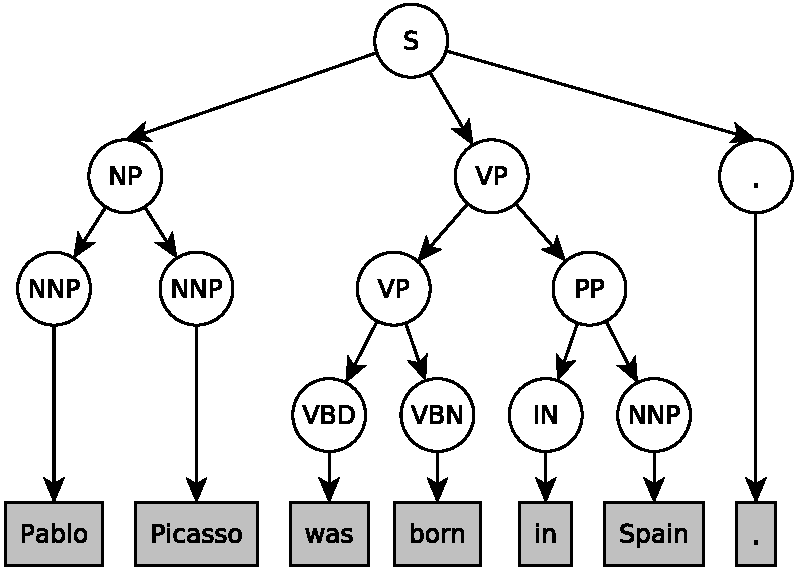
\includegraphics[width=0.62\textwidth]{images/parse-tree.pdf}
    \caption{Syntax tree}
    \label{fig:parse-tree}
  \end{figure}
\end{myItemize}

\noindent
Semantic information which can be used to define patterns are:
\begin{myItemize}
\item Named entities and their types, discovered by named entity recognition described in \autoref{sec:terms-extraction}. Example for the same sentence as in the paragraph above:
\begin{code}
[Person| Pablo Picasso] was born in [Location| Spain]
\end{code}

\item \emph{Semantic role labels} which mark predicate of the sentence and its arguments -- agent (subject), patient (object), cause, purpose, manner, location, time etc.
Semantic roles can be identified using statistical classifier \cite{semantic-role-labelling}.
\begin{code}
[agent| Pablo Picasso] [predicate| was born] [location| in Spain]
\end{code}

\item Semantic relations between words, such as \emph{hypernymy}, i.e. being a super-class (e.g. \emph{animal} as a hypernym for \emph{dog}). These relations between words can be found in \emph{WordNet} \cite{wordnet}.
\end{myItemize}


\subsection*{Examples of transformation rules}

The simplest pattern is for the fill-in-the-blank questions
(used for example by Agarwal and Mannem \cite{question-gen-textbooks}):
\begin{code}
Pattern: beforeTerm term afterTerm.
<*\arrowlinesplit*>
Question: beforeTerm <*\sentenceGap*>afterTerm
Answer: term
\end{code}
\transformationExample%
{The Southern Chinese martial art Hung Ga is based on the movements of the tiger and the crane.}%
{The Southern Chinese martial art \sentenceGap is based on the movements of the tiger and the crane.}%
{Hung Ga}

\noindent
Typical example of a mostly syntactic approach,
with a little bit help of the semantics (using WordNet) to create the final question
\cite{question-gen-mitkov}:
\begin{code}
Pattern: [NP subject] [VP verb] [NP object].
<*\arrowlinesplit*>
Question: <*\emph{Which}*> hypernym(subject) verb object<*\emph{?}*>
Answer: subject
\end{code}
\transformationExample{Logic studies reasoning.}{Which discipline studies reasoning?}{logic}

\noindent
The following example shows that sometimes, questions might be generated just from a phrase, instead of the full sentence and it also makes use of named entities \cite{mentor}.
\begin{code}
Pattern: [NP object] [VBN predicate] <*\emph{by}*> [Human subject]
<*\arrowlinesplit*>
Question: <*\emph{Who}*> pastTense(predicate) object<*\emph{?}*>
Answer: subject
\end{code}
\transformationExample%
{... Hamlet, written by Shakespeare ...}%
{Who wrote Hamlet?}%
{Shakespeare}

\noindent
Some connectives (because, so that, since, when, for example, ...) can be used to generate questions
\cite{question-gen-connectives, questions-wolfe}.
\begin{code}
Pattern: A, <*\emph{because}*> B.
<*\arrowlinesplit*>
Question: <*\emph{Why}*> questionForm(A)<*\emph{?}*>
Answer: Because B.
\end{code}
\transformationExample%
{Photosynthesis is important, because it produces oxygen.}%
{Why is photosynthesis important?}%
{Because it produces oxygen.}

\noindent
Function \texttt{questionForm(A)} searches for an auxiliary verb in \texttt{A} and if it finds one, it moves the auxiliary verb to the front.
If there is no auxiliary verb in the sentence, it adds appropriate auxiliary verb to the beginning of the sentence based on the tense of the main verb and the main verb is substituted for its base form (bare infinitive).
If the main verb is \emph{to be} (as in our example), it is moved to the front without adding any auxiliary verb.

\noindent
As mentioned above, semantic role labels might be used to describe patterns \cite{question-gen-mannem, questions-eval}.
\begin{code}
Pattern: <*\emph{By}*> manner, agent predicate patient.
Filter: manner <*\emph{contains gerundium}*>
<*\arrowlinesplit*>
Question: <*\emph{How}*> questionForm(agent, predicate) patient<*\emph{?}*>
Answer: <*\emph{by}*> manner
\end{code}
\transformationExample%
{By reducing halting problem to problem X, one can show undecidability of the problem X.}%
{How can one show undecidability of the problem X?}%
{by reducing halting problem to problem X}

\noindent
Even more sophisticated patterns can be created using syntax trees \cite{question-gen-ceist, question-overgenerating-rating}.

%\subsection*{Automatic patterns discovery}
In most tools, transformation rules were created manually.
However, machine learning can be put into use to discover them automatically.
\textit{The-Mentor} system \cite{mentor}
uses a machine learning technique of \textit{bootstrapping} \cite{question-answering-bootstrapping},
together with the \textit{QuestionBank}, a corpus of 4000 parse-annotated questions \cite{question-bank},
and the large amount of the information on the Web via \textit{Google} search
to find syntactic patterns automatically from a few question-answer seed pairs.
They have discovered more than 1000 unique patterns, which is many more than tools with manually created patterns use. This allows for more specific patterns, such as the following:
\begin{code}
Pattern: [NP subject] [VBD aux] [VBN verb] <*\emph{in}*> [Location:Country| X].
<*\arrowlinesplit*>
Question: <*\emph{In which country}*> aux subject verb<*\emph{?}*>
Answer: X
\end{code}
\transformationExample%
{Pablo Picasso was born in Spain.}%
{In which country was Pablo Picasso born?}%
{Spain}


% ---------------------------  SECTION  ---------------------------
\section{Creating Exercises from Knowledge Graph}
\label{sec:exercises-from-knowledge-graph}

In this section, we will consider the situation when we have built knowledge graph
and want to create exercises from it, instead of from the original text.
Similarly as with the text, the question generation tool can take a fact one by one
and transform it to the question if possible.
For example, fact \texttt{(Alan Turing, birthDate, 23 June 1912)} leads to the question
\textit{When was Alan Turing born?} with the correct answer \textit{1912}.
However, there are some predicates which are not suitable for creating questions from them,
such as \texttt{rdfs:label} or \texttt{rdf:comment} and these need to be filtered.

This approach of transforming a single fact at a time was used in \textit{OntoQue} \cite{ontoque}.
OntoQue supports 3 types of exercises: multiple choice question, true/false and fill-in-the-blank.
Fill-in-the-blanks are created simply by removing subject or object from the fact.
Multiple-choice-questions are fill-the-blanks with 4 provided choices.
As distractors, subjects or objects of the same type as the removed one are used.
Finally, true statements in true/false questions are just unmodified facts from the knowledge graph,
while false statements are created by replacing subject or object for a different one (suitable alternative is found in the same way as the distractors for multiple choice questions).

OntoQue uses \texttt{rdf:label} property to transform facts into sentences,
so the quality of the generated questions depends on the quality of the labels.
Consider two situations shown in \autoref{fig:rdf-graphs-labels}.
From the left graph, OntoQue could generate fill-in-the-blank question
\emph{Alan Turing was born in \sentenceGap},
while the right graph would be transformed into the question
\emph{Alan Turing birth date \sentenceGap}
Another possible problem could be with the answer, sometimes it needs to be modified
(in our example \emph{1912-06-23} could be simplified to \emph{1912}).

\begin{figure}[h]
  \centering
  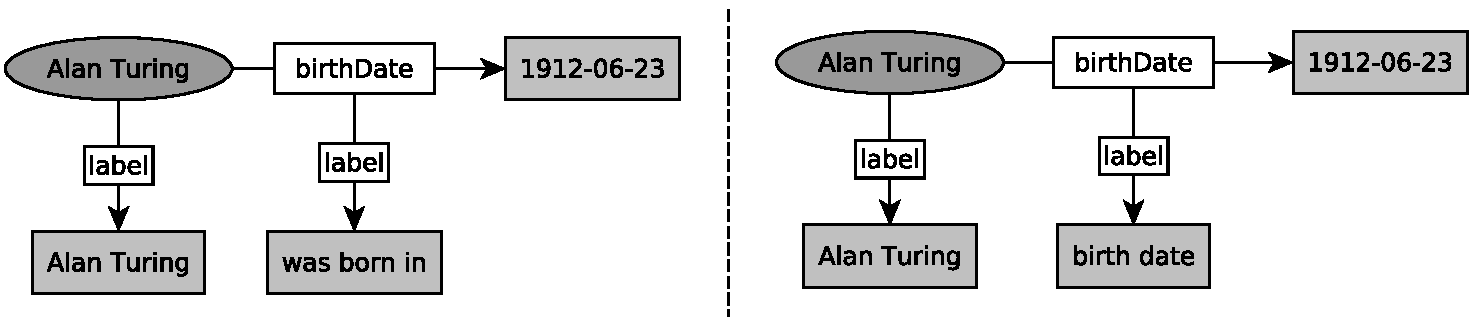
\includegraphics[width=\textwidth]{images/rdf-graph-labels-comparision.pdf}
  \caption{Labels}
  \label{fig:rdf-graphs-labels}
\end{figure}

For this reason we might want to use more specific patterns to influence transformation from facts to sentences and simplify answers. For convenient retrieval of information from a knowledge graph, we can use SPARQL which was described in \autoref{sec:sparql}.
As a simple example, rule for \emph{When was X born?} question would look like this:
\begin{code}
PREFIX ont: <http://dbpedia.org/ontology/>
PREFIX rdfs: <http://www.w3.org/2000/01/rdf-schema#>
SELECT ?subjectName ?birthDate
WHERE {
  ?subject ont:birthDate ?birthDate ;
      rdfs:label ?subjectName .
}
<*\arrowlinesplit*>
Question: <*\emph{When was}*> subjectName <*\emph{born?}*>
Answer: parseYear(birthDate)
\end{code}

\noindent
The following transformation would generate questions about start dates of all events in the knowledge graph.
\begin{code}
PREFIX ont: <http://dbpedia.org/ontology/>
PREFIX rdfs: <http://www.w3.org/2000/01/rdf-schema#>
SELECT ?eventName ?date
WHERE {
  ?event a ont:Event ;
    rdfs:label eventName ;
    ont:startDate ?date .
}
<*\arrowlinesplit*>
Question: <*\emph{When did}*> eventName <*\emph{happen?}*>
Answer: date
\end{code}

\noindent
But the great thing about the knowledge graph is that we can select more facts and then ask a question which span more than one sentence, such as
\textit{Could hypothetically Leonhard Euler meet Carl Friedrich Gauss?}
This transformation is described in the following example.
\begin{code}
PREFIX ont: <http://dbpedia.org/ontology/>
SELECT ?name1 ?birth1 ?death1 ?name2 ?birth1 ?death2
WHERE {
  ?person1 a ont:Person ;
      rdfs:label name1 ;
      ont:birthDate ?birth1 ;
      ont:deathDate ?death1 .
  ?subject2 a ont:Person ;
      rdfs:label name2 ;
      ont:birthDate ?bith2 ;
      ont:deathDate ?death2 .
}
<*\arrowlinesplit*>
Question: <*\emph{Could hypothetically}*> subject1 <*\emph{meet}*> subject2 <*\emph{?}*>
Answer: bool(birth2 <*$\leq$*> death1 <*$\land$*> death1 <*$\geq$*> birth2)
\end{code}


% ---------------------------  SECTION  ---------------------------
\section{Distractor Selection}
\label{sec:distractors}

It is important to present a multiple-choice question with competitive \textit{distractors}.
As shown by experiments performed by Little and Bjork \cite{optimizing-multiple-choice}, multiple choice questions with competitive incorrect alternatives not only help to remember the correct answers to the original questions, but they also improve later performance on the previously non-tested questions for which these alternatives may be the correct answers. If the alternatives are not competitive, a student can recognize the correct answer without retrieval, just by pattern matching.
%As an example, consider the following multiple choice question:
As an example, consider exercise \ref{exrc:noncompetitive}.
\begin{exercise}
\caption{Question with noncompetitive alternatives}\label{exrc:noncompetitive}
  \begin{question}
  Lincoln was assassinated by \sentenceGap , a Confederate sympathizer.
  \begin{choices}
    \choice Emancipation Proclamation
    \choice John Wilkes Booth
    \choice Illinois
    \choice Department of Agriculture
  \end{choices}
  \end{question}
\end{exercise}

\noindent
Clearly, the student does not need to remember who assassinated Lincoln to answer this question correctly and they are also not forced to retrieve any knowledge about alternatives.
Of course, this was an extreme example to illustrate the point -- you definitely would not come across such poor distractors in manually created multiple-choice questions.
%Now take a look at the following question:
Compare the previous question to the exercise \ref{exrc:competitive}.
\begin{exercise}
\caption{Question with competitive alternatives}\label{exrc:competitive}
  \begin{question}
  Lincoln was assassinated by \sentenceGap , a Confederate sympathizer.
  \begin{choices}
    \choice Thomas N. Conrad
    \choice Robert E. Lee
    \choice John Wilkes Booth
    \choice Ward Hill Lamon
  \end{choices}
  \end{question}
\end{exercise}

\noindent
This questions is much more likely to force student to retrieve knowledge about John Wilkes Booth as well as about other alternatives.
Little and Bjork also showed that competitive distractors are not confused with correct answers in later questions more often than noncompetitive distractors.

The consequences are clear -- when creating a multiple-choice question, we should try to find distractors which are as competitive as possible,
which is what most of the current question generation tools do
\cite{question-gen-mitkov, question-gen-textbooks, mentor}.
Common strategies for distractor selection are:
\begin{myItemize}
\item \textbf{Named entities from the text}\\
  One possibility is to use named entities from the text discovered by named entity recognition (\autoref{sec:terms-extraction}). As distractors, named entities of the same type are chosen (e.g. if the correct answer is person, choose people as distractors). This approach was used for example in the Mentor \cite{mentor}.
As an alternative to common types, common context can be used to select appropriate distractors.
Agarwal \cite{question-gen-textbooks} uses features such as comparison of words and their POS tags before and after the correct answer and the distractor or frequency of common words in the question sentence and a sentence with the distractor.

\item \textbf{Subjects in the knowledge graph}\\
In the knowledge graph, subjects play similar role as the named entities in the text.
The difference is that usually one subject has many types.
(For example, the record about \emph{Abraham Lincoln} in DBpedia contains more than 50 types, including
\emph{agent}, \emph{person}, \emph{office holder}, \emph{president of the United States} and \emph{people murdered in Washington, D.C.})
Several strategies were proposed to select the most competitive distractors in the knowledge graph \cite{ontoque, question-gen-domain-ontologies}. One of them is to select a subject of the same type as the correct answer. If there are many of them, we can prefer those which have more common types.

\item \textbf{Named entities from external sources}\\
  Using \textit{WordNet} \cite{wordnet} or a knowledge base, we can find similar terms, even if they are not in the text. For example, Mitkov et al. \cite{question-gen-mitkov} use \textit{coordination relation} in WordNet (coordinates are words sharing at least one hypernym) to find appropriate distractors for given term. If more coordinates were found in WordNet, the ones which occur in the text are preferred.

\item \textbf{Correct answer modification}\\
  If the correct answer is a numerical expression, we can easily obtain distractors by changing the date or value by some partially random relative shift or (sub)multiplication
\cite{question-gen-domain-ontologies}.
For instance, if the correct answer is $1616$ the distractors generated by multiplying the correct answer by $0.92$, $0.95$ and $1.04$ would be $1487$, $1535$ and $1680$.
\end{myItemize}

\noindent
All these strategies work only if the correct answer is a named entity or a single word.
If the correct answer is a full clause
(e.g. \emph{Why is photosynthesis important? / Because it produces oxygen.}),
generating meaningful and competitive distractors is much harder.
Simple (but not very good) way to find at least some distractors would be to use the correct answers of the generated questions of the same question type.


% ---------------------------  SECTION  ---------------------------
\section{Question Ranking and Filtering}
\label{sec:questions-ranking-filtering}

Common strategy in the question generation tools
is to overgenerate questions and then filter them
\cite{mentor, question-gen-mannem, question-overgenerating-rating, questions-wolfe}.
The goal of the filtering is to discard questions which are:

\begin{myItemize}
  \item invalid (e.g. because they contain anaphoric references, such as \emph{Where is there?}),
  \item irrelevant to the topic,
  \item too easy (e.g. because of noncompetitive distractors).
\end{myItemize}

As an alternative to direct filtering,
we can rank questions first and then select $N$ best questions
(e.g. Mannem \cite{question-gen-mannem} selects $6$ best questions per a paragraph).
Ranking allows to separate the task of estimating parameters and the task of selecting questions for the student based on the already answered questions,
%deciding which question is the best for the student right now,
i.e. it allows for adaptive practice (\autoref{chap:practice}).
We can even separately rank various parameters of questions, such as probability of correctness (validity), relevance and difficulty.

Both filtering and ranking can be implemented either via heuristic decisions
or via a machine-learning based classifier.
Some possible heuristic criteria to discard generated questions are \cite{questions-wolfe}:
\begin{myItemize}
\item Question or answer is too long.
\item Question contains word \emph{and}, colon or quotes.
\item The first word in the answer is a relative pronoun.
\end{myItemize}

Mannem \cite{question-gen-mannem} uses heuristic ranking,
with depth of the predicate from which is the question generated as a primary criterion
(to penalize questions from subordinate clauses)
and the number of pronouns as a secondary criterion (to penalize possible anaphoric references).

Heilman \cite{question-gen-heilman} trained a machine learning-based classifier for question ranking using features such as:
\begin{myItemize}
\item question length,
\item which wh-word (who, where, when, ...) was used (if any),
\item includes negation (no, not, never)? (binary feature),
\item likelihoods of a question would appear in a text according to an unigram and a trigram language models,
\item number of proper noun, pronouns, adjectives, etc.
\end{myItemize}

The presented rankers are primarily concerned with correctness (validity) of generated questions.
However, for the adaptive practice, difficulty ranking is necessary as well.
Smartoo uses a simple heuristic for difficulty ranking, which is described in \autoref{sec:smartoo-exercises-grading}.


% ===========================  CHAPTER ===========================
\chapter{Adaptive Practice}
\label{chap:practice}

The goal of \emph{computerized adaptive practice} \cite{adaptive-practice-irt-math}
is to make the practice as efficient as possible.
This is related to, but different from the \emph{computerized adaptive testing} \cite{computerized-adaptive-testing},
which aims at precise and reliable measuring of student's knowledge (or skill).
There are many systems providing practice customized to the learner,
these systems are called \emph{intelligent tutoring systems} \cite{tutoring-systems-behavior}.
Some of them focus on the procedural knowledge (such as solving math problems) \cite{adaptive-practice-irt-math},
other on adaptive practice of facts \cite{slepe-mapy}.

For practice to be efficient, it is important to balance difficulty of the task with respect to the learner.
If the practice is too easy, the learner doesn't learn anything new and quickly becomes bored.
On the other hand, if it is too difficult, the learner becomes anxious and frustrated.
Hence, the key of efficient adaptive practice is to find the optimal difficulty --
Thomas Butt talks about ``the sweet spot of learning'' \cite{adaptive-practice}.
Generally, the ideal state of absolute immersion, focus and enjoyment is called \emph{flow} \cite{flow}.

\begin{figure}[h]
  \centering
  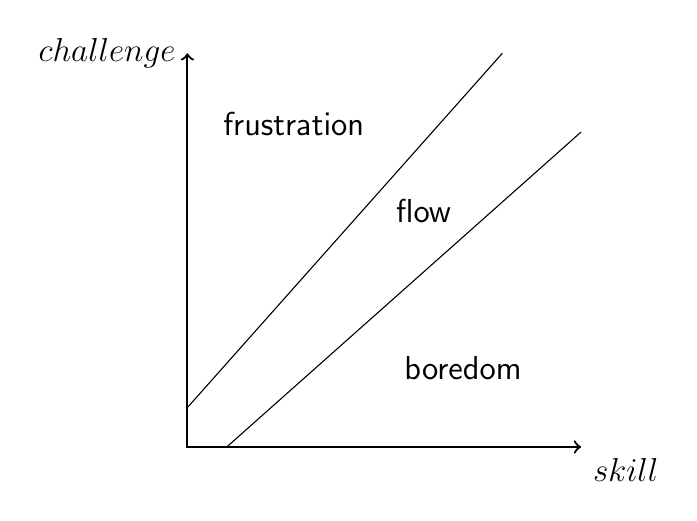
\begin{tikzpicture}[font=\sffamily,xscale=5, yscale=5]
  \large
  %\draw [lightgray, fill=gray] (0,0) -- (0.1,0) -- (1,0.8) -- (0.8,1) -- (0,0.1) -- (0,0);
  \draw (0.1,0) -- (1,0.8);
  \draw (0,0.1) -- (0.8,1);
  \draw [thick, <->] (0,1) node [left] {$challenge$} -- (0,0) -- (1,0) node [below right] {$skill$};
  \node at (0.27,0.82) {frustration};
  \node at (0.6,0.6) {flow};
  \node at (0.7,0.2) {boredom};
  \end{tikzpicture}
  \caption{Relationship between challenge and skill.}
  \label{fig:flow}
\end{figure}

Intelligent tutoring systems use answers (attempts) of learners to estimate both knowledge (skill) of each learner and the difficulty of all facts (tasks).
As most people use these tutors repeatedly and not only once, the process of learning can be also captured
and the systems may have special estimate parameter for each learner-fact pair \cite{slepe-mapy}.

Our situation is, however, different, as there is no limited set of facts.
In each practice session, tens (or even hundreds) of new questions are generated
and we don't know much neither about the questions, nor about the learner's knowledge of the topic.
As there is usually so many generated questions, we can't ask learner all of them,
but carefully select just a few questions, which are the most relevant to the learner and are not too easy nor too difficult.
The generated questions are brand-new, so we necessarily need to rank them for relevance and difficulty estimation (and possibly other attributes as well) as described in \autoref{sec:questions-ranking-filtering},
otherwise there is no way to distinguish between generated questions.

Having the limitations in mind, we can now formulate the goal of the adaptive practice in the settings of the automatically generated questions.
The system shall ask questions, which are relevant to the topic, ideally covering the whole article and which are not answerable without thinking. Furthermore, the system shall attempt to estimate the global knowledge of the student about the topic as quickly as possible and using this estimate, prefer adequately difficult questions, so that the student is neither bored by too easy questions, nor frustrated from too difficult questions.

In \autoref{sec:knowledge-estimation}, I describe several common models of a student used to estimate one's knowledge, then I briefly mention dynamic adjustment of target difficulty (\autoref{sec:target-difficulty}),
and finally I discuss the selection of the best question (\autoref{sec:question-selection}).


% ---------------------------  SECTION  ---------------------------
\section{Knowledge Estimation}
\label{sec:knowledge-estimation}

The collection of persistent information about the student which is used to decide which skill to practice next is called the \textit{student model} \cite{tutoring-systems-behavior}.
It may include information about which skills have been mastered by the student
(and to which extent),
or even enjoyment and motivation of the student \cite{learner-skill-models-review}.

In the settings of facts practicing, student model is used to estimate the probability that given student knows a given fact \cite{slepe-mapy}.
The most common student models for factual knowledge are described
in the following paragraphs.
\begin{myItemize}
\item \textbf{Logistic model}\\
  One-parameter logistic model is the basic model of student in the
  \emph{item response theory} \cite{visual-irt}.
  This model uses logistic function with a parameter $d$, which denotes the difficulty of the fact.
  The probability, that the student with knowledge $k$ knows a fact with difficulty $d$ is given by the formula:
  \begin{equation}\label{eq:logistic}
  P(k, d) = \frac{1}{1 + e^{-(k - d)}}
  \end{equation}
  The logistic function is suitable for probability modeling, because it ranges from $0$ to $1$ for any possible input.
  In case of multiple choice questions, we need to adjust the formula a little bit to account for the possibility of guessing.
  With $n$ options, the probability of correct guess is $\frac{1}{n}$.
\begin{equation}\label{eq:logistic-mcq}
P(k, d, n) = \frac{1}{n} + \left( 1 - \frac{1}{n} \right) \cdot \frac{1}{1 + e^{-(k - d)}}
\end{equation}
Given enough data, model parameters can be estimated using
one of \emph{maximum likelihood estimation} algorithm \cite{irt-theory-and-practice}.
However, since we use generated questions, we do not have any data about students' answers to them.
That is why we need to have some heuristic estimates of difficulty.
Student knowledge is then estimated using questions he or she already answered and their difficulties,
according to \emph{maximum likelihood principle}, i.e. the knowledge level is selected which maximizes the likelihood of the student history.
Although this cannot be solved analytically, fast numeric methods can be used,
e.g. \emph{Newton-Raphson method} \cite{irt-ability-estimation}.

\begin{figure}[h]
  \centering

  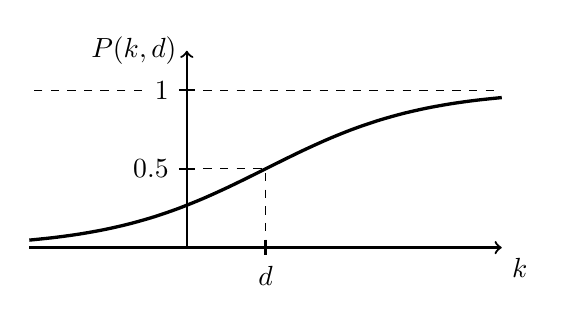
\begin{tikzpicture}[domain=-2:4, smooth, samples=20, scale=1]
  \draw [thick, ->] (-2,0) -- (4,0) node [below right] {$k$};
  \draw [thick, ->] (0,0) -- (0,2.5) node [left] {$P(k,d)$};
  \draw [thick] (-0.1,1) node [left] {$0.5$} -- (0.1,1);
  \draw [thick] (-0.1,2) node [left] {$1$} -- (0.1,2);
  \draw [thin, dashed] (0,2) -- (4,2);
  \draw [thin, dashed] (0,1) -- (1,1) -- (1, 0);
  \draw [thin, dashed] (-0.57,2) -- (-2,2);
  \draw [thick] (1,0.1) -- (1,-0.1) node [below] {$d$};
  \draw [very thick] plot (\x, {2 / (1 + exp(1 - \x))});
  \end{tikzpicture}
  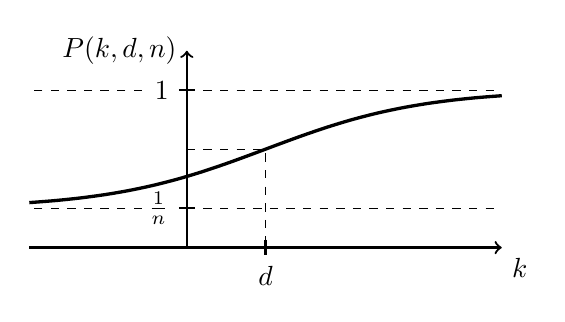
\begin{tikzpicture}[domain=-2:4, smooth, samples=20, scale=1]
  \draw [thick, ->] (-2,0) -- (4,0) node [below right] {$k$};
  \draw [thick, ->] (0,0) -- (0,2.5) node [left] {$P(k,d,n)$};
  \draw [thick] (-0.1,2) node [left] {$1$} -- (0.1,2);
  \draw [thick] (-0.1,0.5) node [left] {$\frac{1}{n}$} -- (0.1,0.5);
  \draw [thin, dashed] (0,2) -- (4,2);
  \draw [thin, dashed] (0,1.25) -- (1,1.25) -- (1, 0);
  \draw [thin, dashed] (-0.57,0.5) -- (-2,0.5);
  \draw [thin, dashed] (-0.57,2) -- (-2,2);
  \draw [thin, dashed] (0,0.5) -- (4,0.5);
  \draw [thick] (1,0.1) -- (1,-0.1) node [below] {$d$};
  \draw [very thick] plot (\x, {0.5 + 1.5 / (1 + exp(1 - \x))});
  \end{tikzpicture}
  \caption{Logistic model without guessing (left) and with guessing (right)}
  \label{fig:logistic-function}
\end{figure}


\item \textbf{Elo model}\\
  Elo model extends the logistic model to capture changing knowledge.
  The model is inspired by the rating of chess players \cite{elo-rating} and interprets each attempt of a student to answer an question as a ``match'' between the student and the question.
  According to the result $R$ of the match (1 for correct and 0 for incorrect answer)
  and the expected result $P(k, d)$
  (computed by the logistic function \ref{eq:logistic}, or \ref{eq:logistic-mcq} for multiple choice questions)
  the knowledge $k$ and difficulty $d$ are updated as follows:
  \begin{equation}\label{eq:elo}
  \begin{array}{l}
      k \gets k + K (R - P(k, d))\\
      d \gets d - K (R - P(k, d))
  \end{array}
  \end{equation}
The difference $(R - P(k, d))$ expresses how much the result was unexpected.
The $K$ parameter influences the weight of the last match to the current estimate.
% NOTE: lze podotknout, ze misto konstanty K se casto pouziva funkce (uncertainty function), mozna citace na Glicko
Although the primary use of Elo model was to describe the process of learning,
it can be also used for the gradual improvements of estimates for prior knowledge of students and difficulty of facts \cite{slepe-mapy}.
However, the constant $K$ is problematic -- if it's too large, estimation is unstable; if it's too small, estimation converges too slowly.
For this reason, instead of a constant, an attenuation function
\begin{equation}\label{eq:attenuation}
  K(m) = \frac{a}{1 + bm}
\end{equation}
($m$ is the order of the match, $a$ and $b$ are fixed parameters) can be used.
The main advantage of using the Elo model to estimate the prior knowledge and difficulties in comparison with the maximum likelihood estimation algorithms is its simplicity and intrinsic online nature.
Experiments suggest that it leads to similar results as the maximum likelihood estimation \cite{slepe-mapy-time-elo}.

\item \textbf{Performance factors analysis}\\
  Performance factors analysis \cite{performance-factors-analysis} is also similar to the logistic model
  and enables to capture learning.
  According to this model, the probability that a student answers correctly to a question
  depends on the difficulty $d$ of the question and number of correct ($a$) and incorrect ($b$) answers of the student to this question in the past. The exact formula is:
  \begin{equation}\label{eq:pfa}
  P(a, b, d) = \frac{1}{1 + e^{-k}}
  \text{~~where~~} k = \alpha \cdot a + \beta \cdot b - d
  \end{equation}
  The main drawback of this model is that it ignores the order of answers,
  so answering firstly 10 times incorrectly and then 10 time incorrectly leads to the same prediction as answering alternately correctly and incorrectly (and while the first case suggests that the student has learned the item, in the second case it's clear that the student hasn't learned it already).
  To take the order of answers into account, performance factors analysis can be combined with the Elo model \cite{slepe-mapy} -- after each answer, estimate of knowledge parameter $k$ is updated according to the rule \ref{eq:elo}.
\end{myItemize}



% ---------------------------  SECTION  ---------------------------
\section{Target Difficulty Adjustment}
\label{sec:target-difficulty}

As we mentioned in the introduction to this chapter,
the key to the efficient practice is to provide the student with adequately difficult questions.
Although the ideal success rate may vary for different people (and even for one person in different conditions),
for simplicity it is usually treated as a constant and set e.g. on 75 \% \cite{slepe-mapy, adaptive-practice-irt-math}.

Experiments performed in the online adaptive system for learning geography facts suggest that the optimal success rate may be 65--70 \% \cite{slepe-mapy-motivation}.
This result was obtained by self-reports of students (after some number of answered questions, students were asked if the practice is ``too easy'', ``appropriate'', or ``too difficult'');
each student was assigned to one of 10 groups with different target probability of correct answer (from 50 to 95 \%).

It was also noticed that the actual success rate is usually higher than the target probability of correct answer.
To approach the desired target success rate more closely, an algorithm was proposed for dynamic adjustment of target difficulty \cite{slepe-mapy-motivation}.
It is based on the idea of \textit{proportional controller}.
If the actual success rate is lower than the target probability of correct answer, the target probability is increased (proportionally to the ``error'').
If the actual success rate is higher, the target probability is proportionally decreased.
The exact adjustment function is shown in \autoref{fig:adjusted-target-probability}.

\begin{figure}[h]
  \centering
    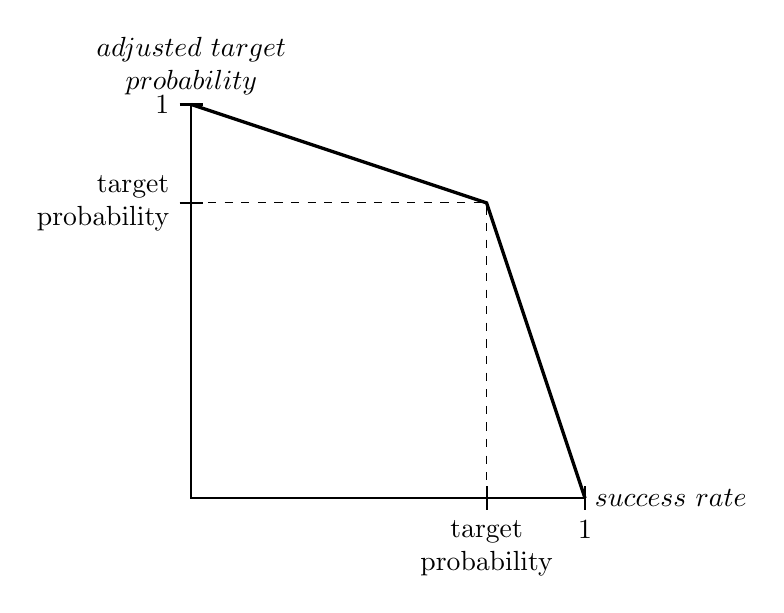
\begin{tikzpicture}[scale=5]
    \draw [thick] (0,1) -- (0,0) -- (1,0);
    \draw (0,1) node [align=center, above] {$adjusted~target$\\$probability$};
    \draw (1,0) node [right] {$success~rate$};
    \draw [very thick] (1,0) -- (0.75,0.75) -- (0,1);
    \draw [thick] (-0.03,1) node [left] {$1$} -- (0.03,1);
    \draw [thick] (-0.03,0.75) node [align=right,left] {target\\probability} -- (0.03,0.75);
    \draw [thick] (1,-0.03) node [below] {$1$} -- (1,0.03);
    \draw [thick] (0.75,-0.03) node [align=center,below] {target\\probability} -- (0.75,0.03);
    \draw [thin, dashed] (0,0.75) -- (0.75,0.75) -- (0.75,0);
    \end{tikzpicture}
  \caption{Function describing adjustment of target probability}
  \label{fig:adjusted-target-probability}
\end{figure}

This dynamic adjustment of target probability proved to be useful -- it increased by 5~\% the set of people who reported that the difficulty is ``appropriate'' \cite{slepe-mapy-motivation}.


% ---------------------------  SECTION  ---------------------------
\section{Question Selection}
\label{sec:question-selection}

In the previous sections, we discussed how to estimate students' knowledge and how to dynamically adjust target difficulty of questions.
Using these two components, we can find the question with the optimal difficulty.
However, several criteria should be considered to select the question which is the most useful for the student and difficulty is just one of them. Let us review the most important criteria.
\begin{myItemize}
  \item \textbf{Relevance}\\
    The question should be relevant to the practiced topic.
    %A possible approach to ranking the relevance of questions was described in \autoref{sec:questions-ranking-filtering}.
    Besides this \emph{objective relevance} which is independent of the student and the practice session,
    there is also what we could call \emph{subjective relevance}, i.e. what concept is the most relevant to the student right now.
    The subjective relevance changes during the practice, as some parts of the article are already practiced and some are not.
    Generally, the most subjectively relevant for the student is
    \emph{the least known concept} \cite{question-gen-adapt-bayes}
    (provided it is also objectively relevant to the topic).

  \item \textbf{Difficulty}\\
    We already discussed that the optimal probability of correct answer is about 70 \% and we also mentioned a method for dynamic adjustment of this target probability (\autoref{sec:target-difficulty}).
    Using a student model (\autoref{sec:knowledge-estimation}) we can estimate the probability that a student would answer given question correctly.
    The more closer is the estimated probability to the target probability, the more is this question preferred.

  \item \textbf{Variability}\\
    Especially important is the variability in the practiced concepts.
    If one concept is practiced in several questions in a row, it gets quickly boring, and it negatively influences both the relevance (as the student would like to practice other concepts from the article as well) and the difficulty (since it is easier to answer questions about the same concept which was already practiced).
    Besides this crucial variability of concepts,
    variability of question types may also help, because diversity increases enjoyment.
    The variability of question types is taken into account e.g. in \emph{Slepé mapy} \cite{slepe-mapy} and \emph{DynaLearn} \cite{question-gen-adapt-bayes}.
\end{myItemize}
Common approach is to use an appropriate scoring function for each of the considered criteria, and then obtain the total score as a linear combination of individual scores \cite{slepe-mapy}.
The question with the highest total score is selected and presented to the student.




% ===========================  CHAPTER ===========================
\chapter{Smartoo Framework}
\label{chap:smartoo}

Smartoo is a framework for question generation and adaptive practice.
It is written in a modular way and decomposes the process into the following components:
\begin{myItemize}
\item \textbf{KnowledgeBuilder} -- takes an article as the input and extracts knowledge, building a RDF graph of facts contained in the article.
\item \textbf{ExercisesCreator} -- creates a set of questions (or possibly other types of exercises) using the built knowledge graph.
\item \textbf{ExercisesGrader} -- ranks generated exercises with respect to attributes such as difficulty or relevance to the original article.
\item \textbf{Practicer} -- controls the practice session itself, i.e. gives the student one exercise at a time based on the previous exercises and answers.
\end{myItemize}
Each component (e.g. \textit{KnowledgeBuilder}) has variable behavior (e.g. \textit{KnowledgeBuilderBehavior}), which is a parametrised code, i.e. an implementation of the behavior (the code) and a set of parameters which the code uses.
Component itself is just a wrapper around the behavior which performs common tasks, most importantly persistence management.
%(For example \textit{KnowledgeBuilder} stores the knowledge graph built byt its behavior.)
At the beginning of each new session, 4-tuple of components with behaviors is chosen.%
%\footnote{The selection is not actualy completely random, behaviors with better performance in the past are preferred over the behaviors with worse performance, see section \autoref{sec:smartoo-behaviors-selection} for details.}
%The described relationships are visualized in \autoref{fig:smartoo-architecture}.

\begin{figure}[h]
  \centering
  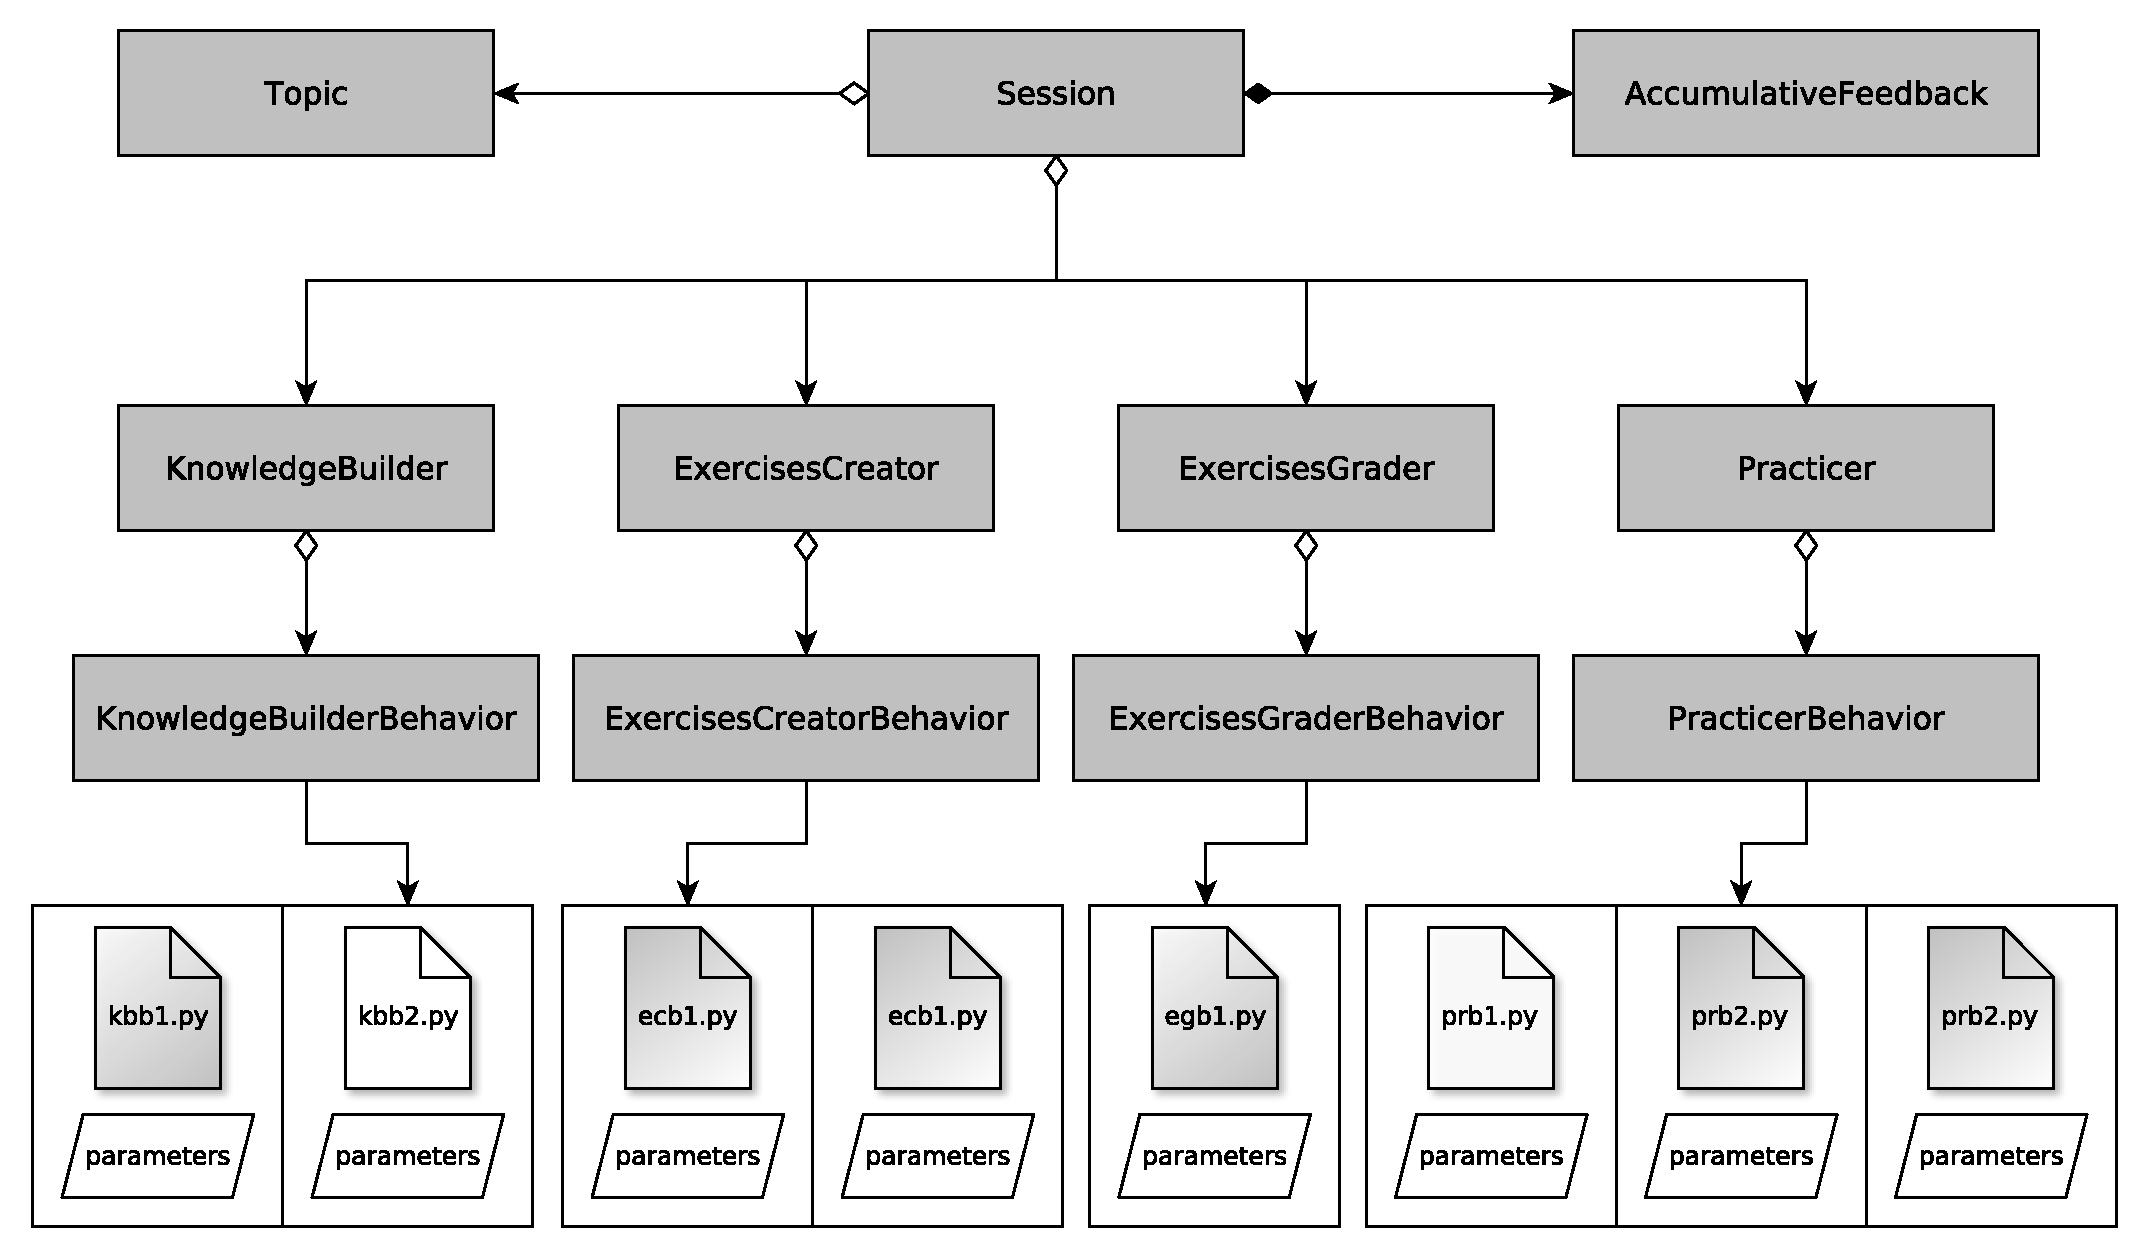
\includegraphics[width=\textwidth]{images/architecture.pdf}
  \caption{Components and behaviors}
  \label{fig:smartoo-architecture}
\end{figure}

The proposed modular design allows for easy integration and testing of new behaviors.
Simple prototype behaviors based on heuristic approaches were implemented.
More sophisticated behaviors will be the subject of future development.

Except from \textit{ExercisesCreator} and \textit{ExercisesGrader},
the components does not communicate with each other directly,
but via results (knowledge graphs and exercises) stored in the database.
The communication and the flow of data is depicted in \autoref{fig:data-flow-diagram}.
Individual processes are triggered by signals from the client.
Time ordering of the signals and processes is shown in \autoref{fig:client-server-communication}
on page~\pageref{fig:client-server-communication}.

\begin{figure}[h]
  \centering
  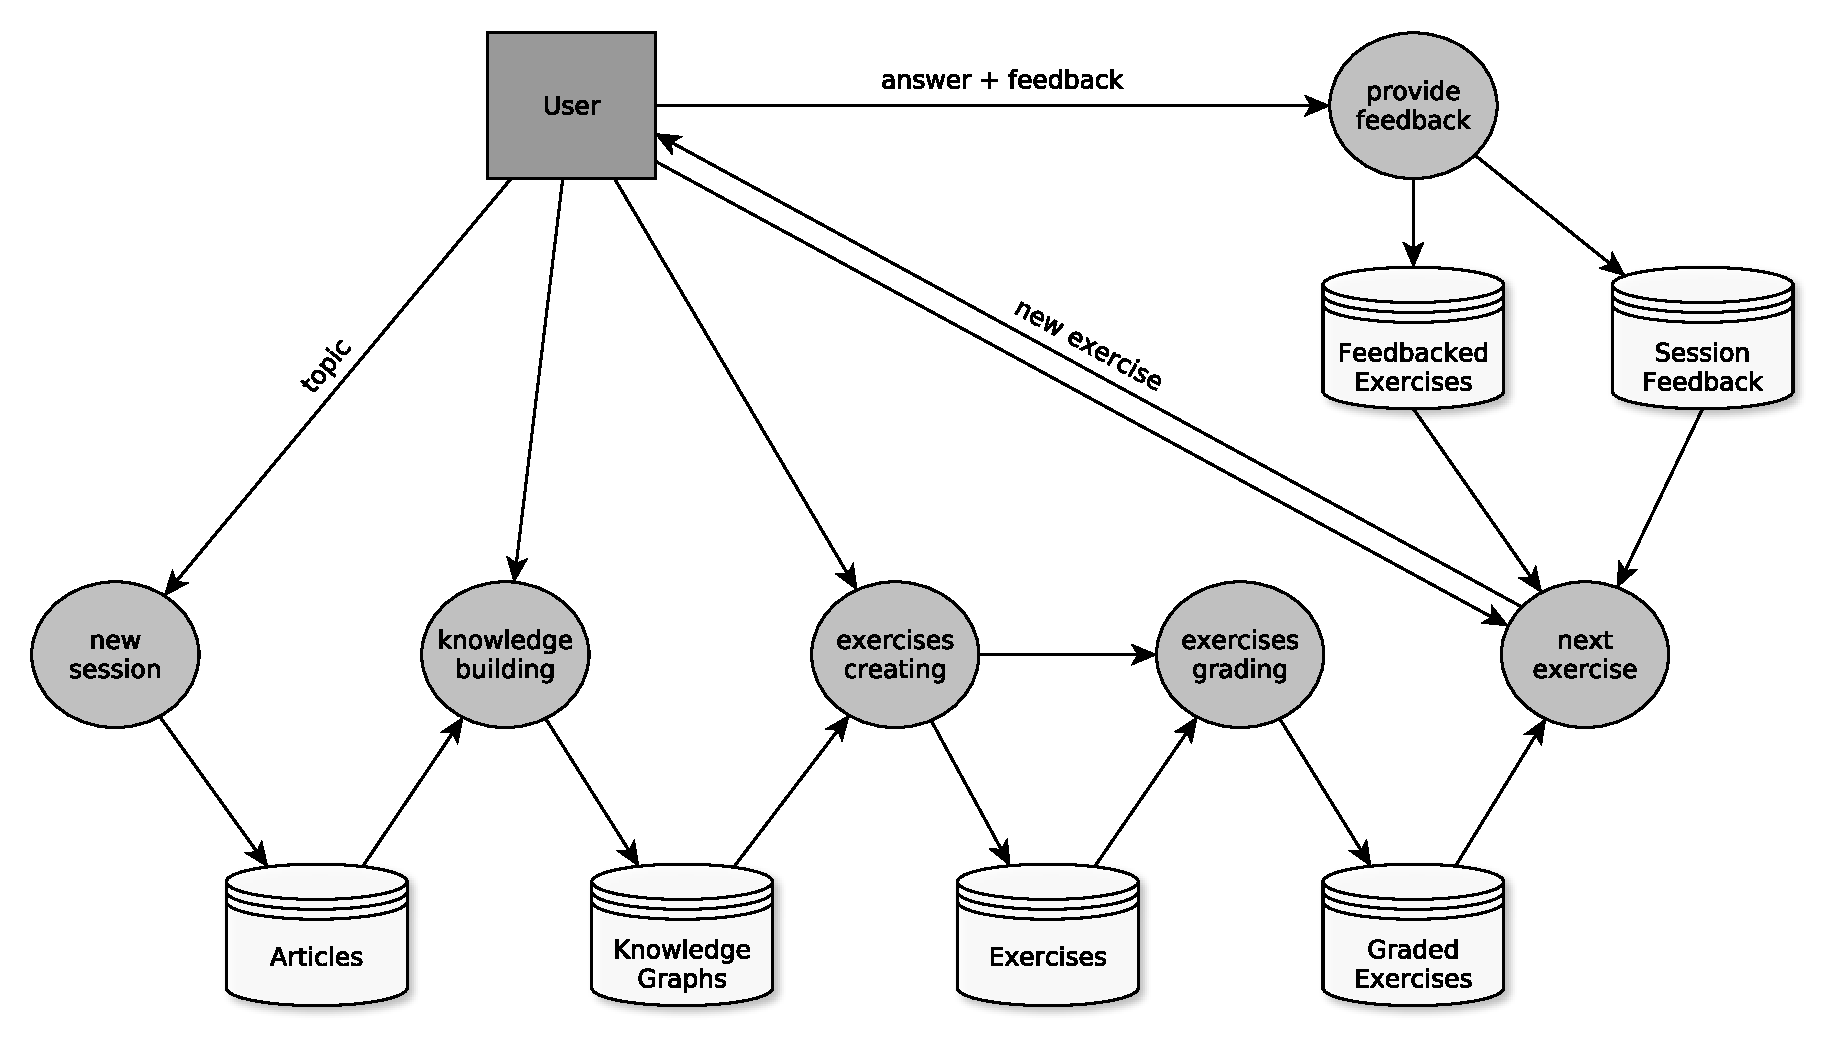
\includegraphics[width=\textwidth]{images/data-flow-diagram.pdf}
  \caption{Data flow diagram}
  \label{fig:data-flow-diagram}
\end{figure}

% ---------------------------  SECTION  ---------------------------
\section{Behaviors Selection}
\label{sec:smartoo-behaviors-selection}

Each session has assigned a \textit{performance} which is computed as a weighted sum of the user final rating and the ratio of exercises marked as invalid or irrelevant.
As we know which behaviors participated in which sessions, we can compute the average performance of a 4-tuple of behaviors $p(x_1, x_2, x_3, x_4)$.

At the beginning of each new session, 4-tuple of behaviors $(k_1, k_2, k_3, k_4)$ ($k_1$ is knowledge builder, $k_2$ exercises creator, etc.) is chosen in a partially random way
which prioritizes behaviors with better performance in the past.
Ideally, the probability of a certain 4-tuple being selected would be proportional to its expected relative performance
(relative to the expected performances of other 4-tuples).
As we do not know the future, our best guess for the expected performance is the performance in the past.
Using conditional probability we can easily derive formulae for probability $P$ of components $(x_1, x_2, x_3, x_4)$ being selected.
I use asterisk ($*$) to denote ``any behavior'', so e.g. $p((x_1, *, *, *))$ means average performance of all sessions in which knowledge builder was $x_1$.
$$
P(k_1 = x_1) = p((x_1, *, *, *)),
$$
$$
P(k_2 = x_2 \mid k_1 = x_1)
  = \frac{P(k_1 = x_1 \land k_2 = x_2)}{P(k_1 = x_1)}
  = \frac{p((x_1, x_2, *, *))}{p((x_1, *, *, *))},
$$
$$
P(k_3 = x_3 \mid k_1 = x_1 \land k_2 = x_2)
  = \frac{P(k_1 = x_1 \land k_2 = x_2 \land k_3 = x_3)}{P(k_1 = x_1 \land k_2 = x_2)}
  = \frac{p((x_1, x_2, x_3, *))}{p((x_1, x_2, *, *))},
$$
$$
P(k_4 = x_4 \mid k_1 = x_1 \land k_2 = x_2 \land k_3 = x_3)
  = \ldots
  = \frac{p((x_1, x_2, x_3, x_4))}{p((x_1, x_2, x_3, *))}.
$$



% ---------------------------  SECTION  ---------------------------
\section{Articles Parsing}
\label{sec:articles-parsing}

If the user requests topic which were never requested before,
the corresponding article is looked up and retrieved from Wikipedia.
Some text preprocessing is performed, e.g. sections without useful content, such as ``See also'', ``External links'' or ``References'', are discarded.
Then the article is parsed into sentence trees with marked terms occurrences.

%\subsection*{Shallow Parsing}
At first, text is split into sentences, each sentence is tokenized
and each token is assigned a part-of-speech tag.
%(\autoref{sec:sentence-transformations}).
    For these natural language processing tasks I have used the \textit{NLTK} (Natural Language Toolkit) library \cite{nlp-python}. NLTK uses \textit{The University of Pennsylvania (Penn) Treebank Tag-set} \cite{penn-tagset}.

\begin{table}[h]
\begin{center}
\begin{tabular}{| l | l | l |}
  \hline
  Tag & Description & Example \\
  \hline \hline
  NN & common noun, singular & house         \\ \hline
  NNP & proper noun, singular & Lincoln     \\ \hline
  DT & determiner & the \\ \hline
  VB & verb, base form & eat \\ \hline
  JJ & adjective & popular \\ \hline
\end{tabular}
\end{center}
\caption{Part-of-speech tags examples \cite{penn-tagset} }
\end{table}

As an example, consider sentence ``Six days after the surrender of Confederate commanding general Robert E. Lee, Lincoln was assassinated byt John Wilkes Booth, a Confederate sympathizer.'' This sentence would be tokenized and tagged as follows:
\begin{code}
[['Six', 'CD'], ['days', 'NNS'], ['after', 'IN'], ['the', 'DT'],
['surrender', 'NN'], ['of', 'IN'], ['Confederate', 'NNP'],
['commanding', 'NN'], ['general', 'NN'], ['Robert', 'NNP'],
['E.', 'NNP'], ['Lee', 'NNP'], [',', ','], ['Lincoln', 'NNP'],
['was', 'VBD'], ['assassinated', 'VBN'], ['by', 'IN'],
['John', 'NNP'], ['Wilkes', 'NNP'], ['Booth', 'NNP'],
[',', ','], ['a', 'DT'], ['Confederate', 'NNP'],
['sympathizer', 'NN'], ['.', '.']],
\end{code}

%\subsection*{Terms Occurences Inference}
In addition to the text of the article, I also retrieve a list of titles of \textit{internal links}, i.e. links to another pages on the Wikipedia.
These link titles can be thought of as terms (as they have their page in an encyclopedia).
The terms are shallowed-parsed (tokenized and tagged)
and their occurrences in the text are inferred.
As there are often hundreds of terms in an article,
I first made a trie from all terms, which then enables to search for all terms simultaneously.
To represent shallowed parsed sentences with marked terms occurrences,
I use shallow sentence trees.
You can see an example of a sentence tree in \autoref{fig:sentence-tree}.
\begin{figure}[h]
  \centering
  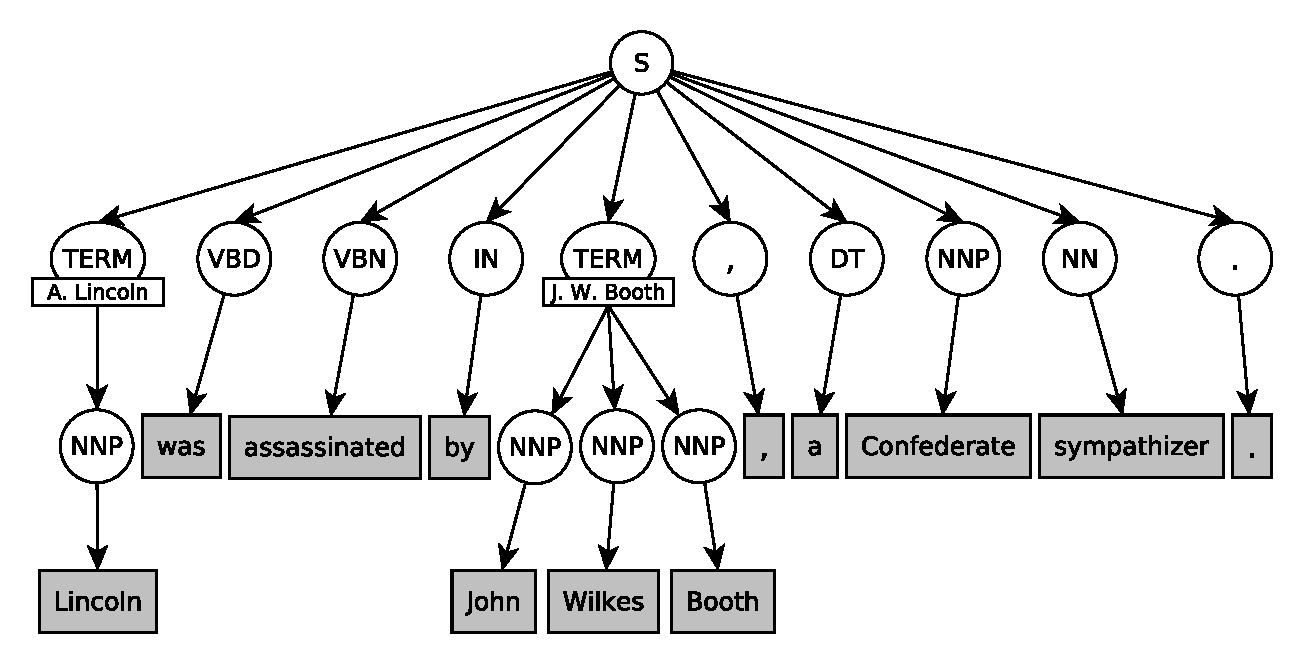
\includegraphics[width=\textwidth]{images/sentence-tree.pdf}
  \caption{Sentence tree}
  \label{fig:sentence-tree}
\end{figure}

% ---------------------------  SECTION  ---------------------------
\section{Knowledge Building}
\label{sec:smartoo-knowledge}

\textit{KnowledgeBuilder} component is responsible for building knowledge graph from a given article.
Knowledge graph is a RDF graph of facts contained in the article.

%\subsection*{Prototype Behavior}

Prototype behavior creates graph of \textit{quasi facts} about terms in sentences.
By the term \textit{quasi fact} I mean some information usable for creating exercises, but not really an elementary unit of knowledge, which ordinary facts should be. The algorithm is simple:
\begin{myEnumerate}
  \item Firstly, an empty graph is created (let us call it $G$).
  \item If it was not already in the past, knowledge graph of the topic term is retrieved from DBpedia (\autoref{sec:knowledge-bases}). All terms in this retrieved knowledge graph and also all terms in the article are added into the graph $G$ together with their types and labels (which are also found using DBpedia).
  \item Then we take each sentence in the article and check if it contains a term and is understandable without a context. The used heuristic is: it contains between 5 and 35 tokens (or 50, depending on the selected parameters), does not contain pronouns, parentheses or quotations or some typical anaphoric words (referring to the context) such as ``this''.
  \item For each sentence which satisfies these conditions, we create an quasi fact about the term in this sentence (and add it to $G$). Each quasi fact consists of several pieces of information: text before the term, text after the term and the term itself (and its label and types). An example of a created quasi fact can be seen in \autoref{fig:quasi-fact}.
  \item Graph $G$ is returned.
\end{myEnumerate}


\begin{figure}[h]
  \centering
  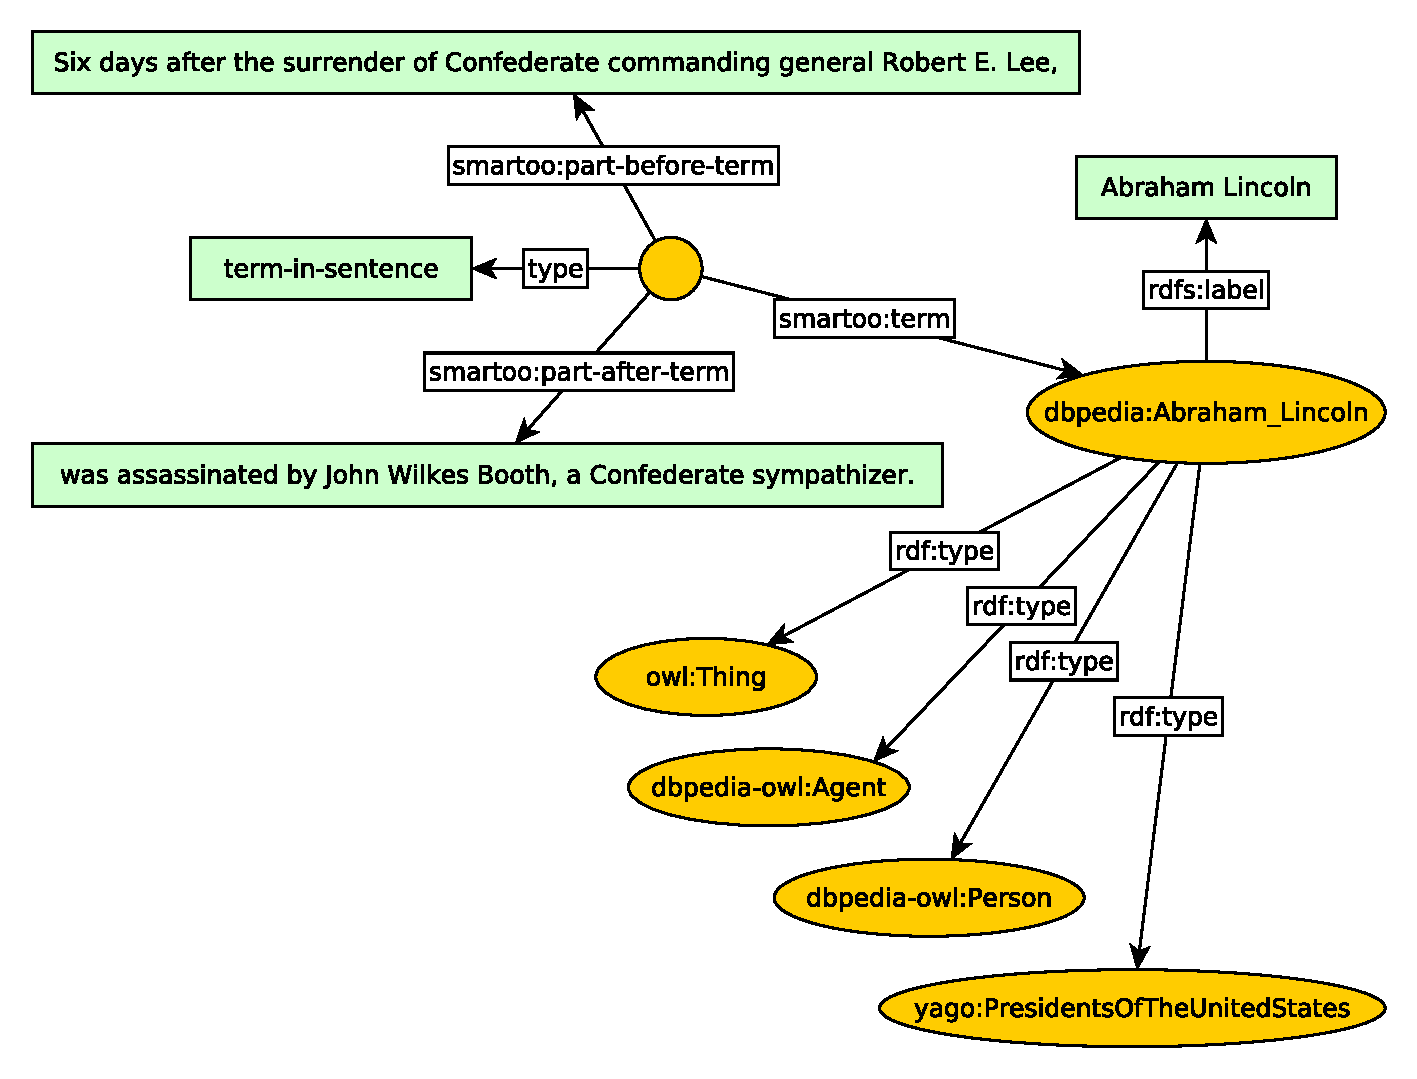
\includegraphics[width=\textwidth]{images/quasi-fact-lincoln.pdf}
  \caption{Example of a quasi fact}
  \label{fig:quasi-fact}
\end{figure}

% ---------------------------  SECTION  ---------------------------
\section{Exercises Creating}
\label{sec:smartoo-exercises}

\textit{ExerciseCreator} component uses built knowledge graph to generate a set of exercises.
Exercises consists of presentation data and semantic information.
\begin{myItemize}
  \item \textbf{presentation data}\\
    Currently the only supported type of exercise is a multiple choice question. Presentation data for multiple choice question consists of a question string, a list of choice labels and a correct answer label (which must be one of the choice labels).
  \item \textbf{semantic information}\\
    Semantic information is used for exercises grading. For this purpose, I decided to use a list of term pairs for which holds, that if the user confuses them, it can lead to an incorrect answer.
    For a multiple choice question with correct answer $A$ and distractors $B$, $C$ and $D$,
    the term pairs are $(A, B)$, $(A, C)$ and $(A, D)$.
\end{myItemize}


Prototype behavior uses all the quasi facts about terms in a sentence and creates \emph{fill in the gap} questions with multiple options.
All quasi facts about terms in sentence can be retrieved from the knowledge graph with the following simple SPARQL query:
\begin{code}
SELECT ?before ?term ?after
WHERE {
    ?quasifact a "term-in-sentence" .
    ?quasifact smartoo:part-before-term ?before .
    ?quasifact smartoo:part-after-term ?after .
    ?quasifact smartoo:term ?term .
}
\end{code}

As we deal with multiple choice question, we also need to select appropriate distractors.
Guided by the results about distractors presented in \autoref{sec:distractors},
the most similar terms to the correct answer are chosen.
Terms similarity heuristics is based on the number of common types
$C(t_1, t_2) = |types(t_1) \cap types(t_2)|$:
$$
sim(t_1, t_2) = 2 \left( \frac{1}{1 + \exp({-|C(t_1, t_2)| / \kappa})} \right) - 1
$$
The constants $\kappa$ influences the speed of convergence to $1$.
Terms without any common type would have $0$ similarity and the more common types they have, the more close to $1$ the similarity is.

As an example, let us look at the exercise created from the quasi fact in \autoref{fig:quasi-fact}. The presentation data looks like this:
\begin{code}
{'question': 'Six days after the surrender of Confederate commanding
              general Robert E. Lee, _______ was assassinated by
              John Wilkes Booth, a Confederate sympathizer.',
'choices': ['Andrew Johnson', 'James Buchanan',
            'Abraham Lincoln', 'Franklin D. Roosevelt'],
'correct-answer': 'Abraham Lincoln'}
\end{code}

%It corresponds to the following presentation of the exercise:
%\begin{exercise}
%\label{exrc:assassination}
%\caption{Example of a created question}
%  \begin{question}
%  Six days after the surrender of Confederate commanding general Robert E. Lee
%  \sentenceGap
%  was assassinated by John Wilkes Booth, a Confederate sympathizer.

%  \begin{choices}
%    \choice Andrew Johnson
%    \choice James Buchanan
%    \choice Abraham Lincoln
%    \choice Franklin D. Roosevelt
%  \end{choices}
%  \end{question}
%\end{exercise}

\noindent
And the respective semantic information is following:
\begin{code}
{'term-pairs': [
    ['Abraham Lincoln', 'Franklin D. Roosevelt'],
    ['Abraham Lincoln', 'James Buchanan'],
    ['Abraham Lincoln', 'Andrew Johnson']]}
\end{code}

% ---------------------------  SECTION  ---------------------------
\section{Exercises Grading}
\label{sec:smartoo-exercises-grading}

\textit{ExerciseGrader} takes an exercise (in particular the semantic part) and assigns it grades for difficulty, relevance to the article and possibly any other attributes, e.g. grammatical correctness probability.

In the prototype behavior, difficulty of an exercise is estimated as the average similarity between all term pairs which can be mistaken.
Similarity of two terms is measured in the same way as during exercise creating (\autoref{sec:smartoo-exercises}).
The value is than normalized to range from $-2$ to $2$
(-2 means extremely simple, 0 average, 2 extremely difficult),
because it is later used by the practicer in the logistic model.

Relevance of the exercise is estimated as the \textit{cosine similarity} measure between the exercise and the article,
i.e. cosine of an angle between the article and the exercise represented as sparse vectors mapping terms to their frequency in the article or the exercise
\cite[][121]{information-retrieval}.
Cosine similarity between two documents (in our case one document is the article $A$ and another is the exercise $E$) is given by the following formula:
$$
similarity(A, E)
= \frac{A \cdot E}{|A| |E|}
= \frac{\sum_{i=1}^{n} A_i E_i}{\sqrt{\sum_{i=1}^{n} A_i^2}\sqrt{\sum_{i=1}^{n} E_i^2}}
$$
where $A_i$ ($E_i$) denotes numbers of occurrences of the $i$-th term in article (exercise).
This measure is commonly used in the information retrieval for estimating similarity between two documents of arbitrary length. The cosine similarity is a real number between $0$ and $1$, the higher it is, the smaller is the angle between documents in the vector space and the more similar the documents are.
In other words, the closer the grade is to 1, the more relevant the exercise is.


\section{Adaptive Practice}
\label{sec:smartoo-practice}

The task of the \textit{Practicer} is to control the practice session itself, i.e. to give the student one exercise at a time based on the previous exercises and answers.
In the prototype behavior, three attributes are considered to select the most suitable exercise:
\begin{myItemize}
  \item relevance to the article,
  \item difficulty (compared to the so far success of the user),
  \item repetitiveness (to not ask about one term over and over again).
\end{myItemize}
Weights of these three attributes in the total score, as well as the target success
are given by the behavior parameters (\autoref{tbl:practicers-parameters}).
\begin{table}[h]
\begin{center}
\begin{tabular}{| c | l | r | r |  r  |  r |  r | r |}
  \hline
           & parameter & \multicolumn{6}{c|}{used values} \\
  \hline
  $\tau$   & target success        & $0.65$ & $0.65$ & $0.65$ & $0.65$ & $0.65$ & $0.65$\\
  $\alpha$ & relevance weight      & $1.00$ & $1.25$ & $1.00$ & $1.00$ & $1.25$ & $1.25$\\
  $\beta$  & difficulty weight     & $1.00$ & $1.00$ & $1.25$ & $1.00$ & $1.00$ & $1.25$\\
  $\gamma$ & repetitiveness weight & $1.00$ & $1.00$ & $1.00$ & $1.25$ & $1.25$ & $1.25$\\
  \hline
\end{tabular}
\end{center}
\caption{Parameters of prototype adaptive practice behavior}
\label{tbl:practicers-parameters}
\end{table}

Relevance of the exercise to the article was computed by \textit{ExercisesGrader}
(\autoref{sec:smartoo-exercises-grading}).
Repetitiveness score is set to the opposite of cosine similarity between the exercise and the exercises already used in the current practice session
(see \autoref{sec:smartoo-exercises-grading} for the explanation and formula of the cosine similarity).

The most interesting part is the difficulty score.
To estimate the probability that the student correctly answers a question with given difficulty (taking into account the possibility of guessing),
I use the logistic model of student as described in \autoref{sec:knowledge-estimation}.
I have also implemented the dynamic adjusting of the target probability \autoref{sec:target-difficulty}.
The difficulty penalization is then set to a difference between the adjusted target probability and the expected probability as calculated by the student model.

Difficulty adjustment is especially useful for students with extremely high knowledge -- the more time student answers correctly, the lower is the adjusted target difficulty, the more difficult exercises are preferred.
In \autoref{fig:knowledge-estimate}, an example of knowledge estimation process during one session is shown.
\autoref{tbl:practice-example} contains detailed information about the same session.

\begin{figure}[h]
\centering
\begin{tikzpicture}[x=1cm,y=2cm,font=\sffamily]
  % axis
  \draw (0,0) -- coordinate (x axis mid) (9,0);
  \draw (0,0) -- coordinate (y axis mid) (0,1.6);
  % ticks
  \foreach \x in {0,...,9}
          \draw (\x,2pt) -- (\x,-4pt)
                  node[anchor=north] {\x};
  \foreach \y in {0,0.4,0.8,1.2,1.6}
          \draw (2pt,\y) -- (-4pt,\y)
                  node[anchor=east] {\y};
  % labels
  \node[below=0.7cm] at (x axis mid) {questions answered};
  \node[align=right,left=1.1cm] at (y axis mid) {knowledge\\estimate};
  % plot
  \draw [thin, dashed] (0,1.2) -- (9.2,1.2) node [right] {true~knowledge};
  \draw plot[mark=square*, mark options={fill=black}] file {knowledge-estimate.data};
\end{tikzpicture}
  \caption{Knowledge estimation during a session}
  \label{fig:knowledge-estimate}
\end{figure}


\begin{table}[h]
\begin{center}
\begin{tabular}{| c | c | c | c | c | c | c |}
  \hline
  & knowledge est. &  target & difficulty & probability est. & true probability & answer\\
  \hline
  $0$ & $+0.000$ & $0.65$ & $-0.2$ & $0.662$ & $0.852$ &  correct   \\
  $1$ & $+0.290$ & $0.52$ & $+0.8$ & $0.531$ & $0.699$ &  incorrect \\
  $2$ & $-0.050$ & $0.69$ & $-0.4$ & $0.690$ & $0.874$ &  correct   \\
  $3$ & $+0.346$ & $0.63$ & $+0.4$ & $0.615$ & $0.767$ &  correct   \\
  $4$ & $+0.760$ & $0.50$ & $+1.4$ & $0.509$ & $0.588$ &  correct   \\
  $5$ & $+1.250$ & $0.41$ & $+1.8$ & $0.524$ & $0.516$ &  correct   \\
  $6$ & $+1.305$ & $0.34$ & $+1.8$ & $0.534$ & $0.516$ &  incorrect \\
  $7$ & $+1.294$ & $0.54$ & $+1.8$ & $0.532$ & $0.516$ &  incorrect \\
  $8$ & $+0.941$ & $0.66$ & $+0.8$ & $0.651$ & $0.699$ &  correct   \\
  $9$ & $+1.191$ & $0.62$ & $+1.2$ & $0.623$ & $0.625$ &  incorrect \\
  \hline
\end{tabular}
\end{center}
\caption{Adaptive practice for a student with knowledge 1.2}
\label{tbl:practice-example}
\end{table}


After the partial scores for relevance, difficulty and repetitiveness are calculated,
they are summed (with weights given by behavior parameters) to obtain the total score.
$$
\text{totalScore} = \alpha \cdot \text{relevanceScore} + \beta \cdot \text{difficultyScore} + \gamma \cdot \text{repetitivenessScore}
$$
An exercise with the highest total score is chosen.





% ---------------------------  SECTION  ---------------------------
\section{Web Interface}
\label{sec:smartoo-web}

%I have created a simple web interface for Smartoo,
%following the \emph{model-view-controller (MVC)} architectural pattern.
The client controls triggering of processes by requests to the server -- start session, build knowledge, create exercises, next exercise (repeatedly) and session feedback.
\emph{Next exercise} requests (with the exception of the first one) have also a feedback from the previous exercise attached to them.
Feedback includes whether the question was answered correctly or incorrectly, and whether the exercise was marked as invalid or irrelevant.
%Each session consists of at most 10 exercises.
After the last exercise, a session feedback form is displayed, prompting user to express his or her overall feeling from the practice session (with 3 choices: ``Bad'', ``So so'', and ``Good'').
A typical sequence of client requests and server responses is shown in
\autoref{fig:client-server-communication} (gray zones denotes computation, black zones waiting for user response).
%The web page design can be seen in \autoref{fig:smartoo-home} and \autoref{fig:question-unanswered}.

\begin{figure}[h]
  \centering
  
\includegraphics[width=0.84\textwidth]{images/home-page.png}
  \caption{Smartoo home page}
  \label{fig:smartoo-home}
\end{figure}

\begin{figure}[h]
  \centering
  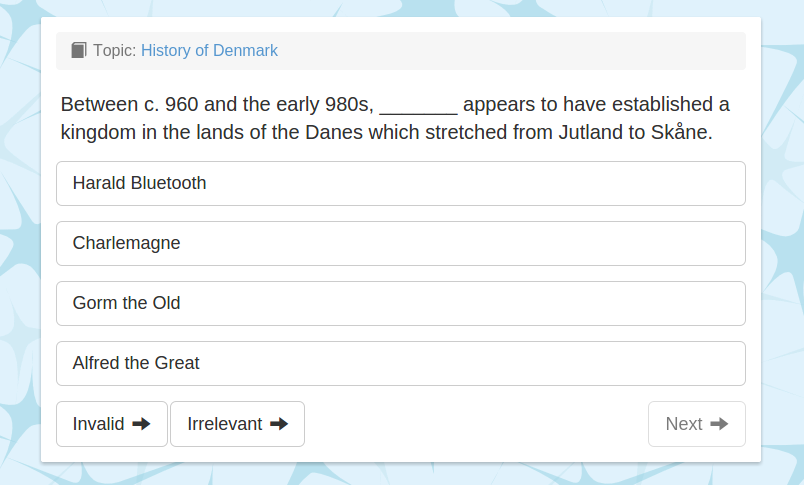
\includegraphics[width=0.84\textwidth]{images/question-unanswered.png}
  \caption{Question about the history of Denmark}
  \label{fig:question-unanswered}
\end{figure}

%\begin{figure}[h]
%  \centering
%  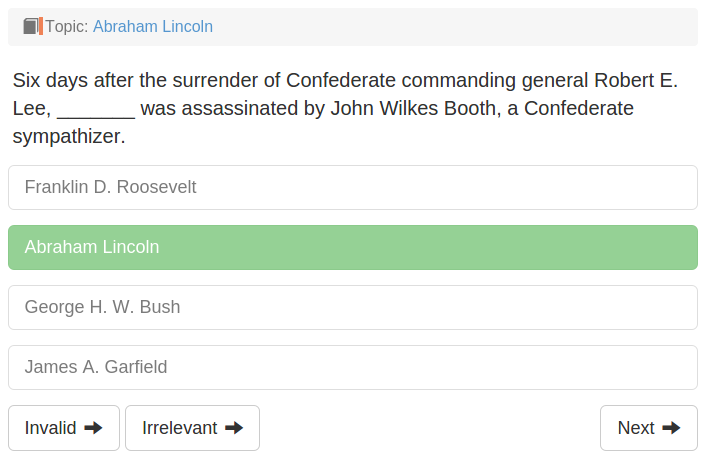
\includegraphics[width=0.9\textwidth]{images/answered-correctly.png}
%  \caption{Correctly answered question}
%  \label{fig:correctly-answered-question}
%\end{figure}

\begin{figure}[h]
  \centering
  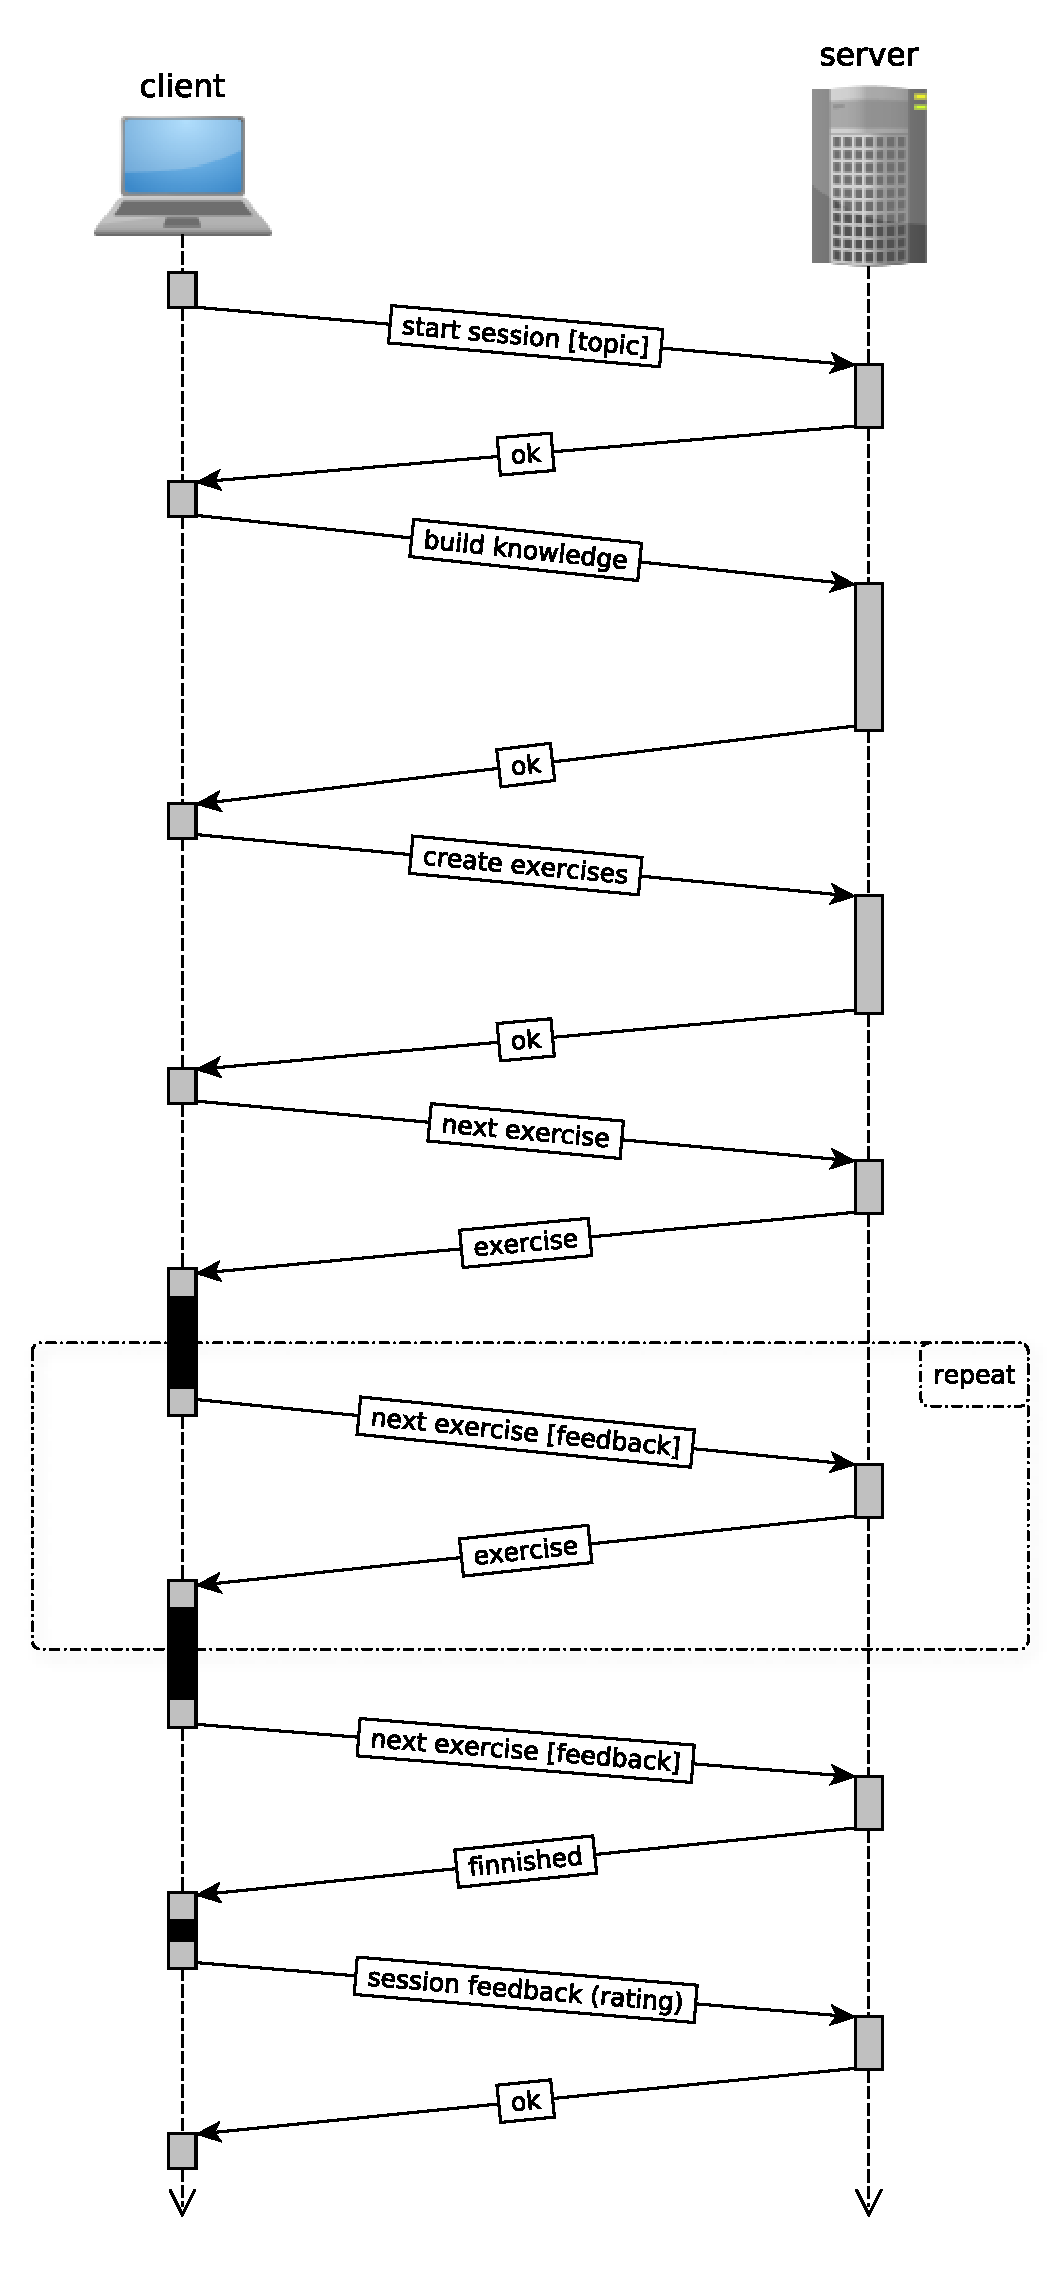
\includegraphics[width=0.66\textwidth]{images/client-server-communication.pdf}
  \caption{Client-server communication}
  \label{fig:client-server-communication}
\end{figure}


% ===========================  CHAPTER ===========================
\chapter{Deployment and Evaluation}
\label{chap:evaluation}

The project structure is described in \autoref{chap:project-structure},
the source code is available from its repository%
\footnote{\url{http://github.com/effa/smartoo}}.
Smartoo has been deployed at \url{http://smartoo.thran.cz}.
In this chapter, I mention a few deployment details
and then I analyze the feedback collected from the users.

% ---------------------------  SECTION  ---------------------------
\section{Used tools and libraries}
\label{sec:tools}

The main tools and libraries used in the project are:
\begin{myItemize}
\item \texttt{Python 2.7}\\
The backend of the application is developed in Python 2.7%
\footnote{\url{https://www.python.org/download/releases/2.7/}}.
To create an isolated Python environment for the project, use \texttt{Virtualenv}%
\footnote{\url{https://virtualenv.pypa.io}}.
After activating a new virtual environment, all necessary Python packages can be installed simply by
command \texttt{pip install -r requirements.txt} executed in the project root directory.
%\begin{code}
%pip install -r requirements.txt
%\end{code}

\item \texttt{Django 1.7}\\
Django%
\footnote{\url{https://www.djangoproject.com/}}
is a Python web framework, using \emph{Model--View--Template} architecture.

%\item \texttt{Jinja2 2.7}\\
%Jinja2%
%\footnote{\url{https://www.djangoproject.com/}}

\item \texttt{NLTK 3.0}\\
NLTK%
\footnote{\url{http://www.nltk.org/}}
(Natural Language Toolkit) is a Python library for natural language processing tasks,
such as tokenization and part-of-speech-tagging.

\item \texttt{SPARQLWrapper 1.6}\\
SPARQLWrapper%
\footnote{\url{http://rdflib.github.io/sparqlwrapper/}}
provides an interface to DBpedia public SPARQL endpoint.

\item \texttt{RDFLib 4.1}\\
RDFLib%
\footnote{\url{https://rdflib.readthedocs.org/}}
is a Python library for working with RDF graphs.

\item \texttt{Wikipedia 1.4}\\
Wikipedia%
\footnote{\url{https://github.com/goldsmith/Wikipedia}}
is a simple Python wrapper for the Wikipedia API.

\item \texttt{SQLite} or \texttt{MySQL}\\
Database is accessed through Django,
so PostgreSQL should probably work as well.
%python manage.py syncdb
%python manage.py migrate

\item \texttt{AngularJS}\\
AngularJS%
\footnote{\url{https://angularjs.org/}}
is a popular JavaScript framework for a simple development of the \emph{Model--View--Controller (MVC)} architecture at the client side.

\item \texttt{Bootstrap}\\
Bootstrap%
\footnote{\url{http://getbootstrap.com/}}
is a HTML and CSS framework for responsive design of the web.
\end{myItemize}





% ---------------------------  SECTION  ---------------------------
\section{Performance Evaluation}
\label{sec:performance-evaluation}

Besides the correct or incorrect answers, Smartoo collects feedback from users through
the ``Invalid'' and ``Irrelevant'' buttons under each generated question,
the practice session final rating form (``bad'', ``so so'' or ``good'')
and an optional ``Write to us'' button.

During testing, 66 practice sessions were taken, with total of 566 questions
(counting only the questions with some response to them, i.e. which were either answered or marked as invalid/irrelevant).
From 544 questions with answers, 394 were answered correctly and 150 incorrectly,
resulting in overall 72 \% success rate.
Thirty seven questions (7 \%) were marked as invalid or irrelevant.
Concerning the practice session final ratings, 24 \% were rated as ``good'', 70 \% as ``so so'' and 6 \% as ``bad''.

Tested version of Smartoo used 2 behaviors for knowledge building.
%, 1 for exercise creating and grading and 6 for practicing.
Knowledge builder behaviors were nearly the same, they only differ in the ``maximum sentence length'' parameter.
Their average performances are shown in \autoref{tbl:builders-performances}.
The behavior using shorter maximum length (30 tokens) performed slightly better.

\begin{table}[h]
\begin{center}
\begin{tabular}{| c | c | c |}
  \hline
      & max length & performance\\
  \hline
  $1$ & $40$ & $0.699$\\
  $2$ & $30$ & $0.738$\\
  \hline
\end{tabular}
\end{center}
\caption{Performances of knowledge builder behaviors}
\label{tbl:builders-performances}
\end{table}

Six different behaviors were used for practicers.
They differ in 3 parameters: relevance weight, difficulty weight and repetitiveness weight.
The used values and their performances are shown in \autoref{tbl:practicers-performances}.
One observation we can made is that setting relevance or difficulty weight higher than repetitiveness weight (behaviors 2 and 3), decreases the performance.

\begin{table}[h]
\begin{center}
\begin{tabular}{| c | c  c  c | c |}
  \hline
      & relevance & difficulty & repetitiveness & performance\\
  \hline
  $1$ & $1.00$ & $1.00$ & $1.00$ & $0.781$\\
  $2$ & $1.25$ & $1.00$ & $1.00$ & $0.671$\\
  $3$ & $1.00$ & $1.25$ & $1.00$ & $0.629$\\
  $4$ & $1.00$ & $1.00$ & $1.25$ & $0.718$\\
  $5$ & $1.25$ & $1.00$ & $1.25$ & $0.783$\\
  $6$ & $1.00$ & $1.25$ & $1.25$ & $0.728$\\
  \hline
\end{tabular}
\end{center}
\caption{Performances of practicer behaviors}
\label{tbl:practicers-performances}
\end{table}

In the written notes from users, some comments appeared several times.
A lot of questions are either quite easy or not completely clear and out of context.
Topic of the article is often used as a correct answer and this usually leads to very simple questions.
Sometimes, the correct answer can be determined just from its type
(e.g. the correct answer is a continent and all distractors are countries).
The practice session progress (in particular, how many questions still remain) should be shown
and a button for terminating the session and jumping back to the home page should be available.



% ===========================  CHAPTER ===========================
\chapter{Conclusions and Future Plans}
\label{chap:future}

There is no doubt that despite the effort of the bachelor thesis,
the question generation remained an open problem of the natural language processing.
Evaluation showed clear limitations of used heuristic approaches.
However, the system was developed with the importance of modularity and extensibility in mind.
New, more sophisticated behaviors for knowledge building, questions creating, questions grading and adaptive practice may be implemented and easily integrated into the current system.

Besides the implementation of advanced behaviors for knowledge extraction and questions creation using machine learning approaches, there are some other improvements I would like to do in the future.
For example, extend the system for the possibility of accepting a plain text, instead of Wikipedia articles.
This would require reasonably good detection of named entities in the text.

%- vyzkouset pouziti jinych bazi znalosti (Freebase)

I would also like to generate different types of questions and exercises,
for example
asking for the cause (why something happens),
open questions with short answers (e.g. who invented something),
matching pairs (scientist -- discovery,  event -- date, ...),
what is on the picture,
ordering time events, etc.
%creation of own multiple choice quesiton

In case of long articles, it could be useful to interleave reading and practice.
It would be also great to make the practice length variable based on the student performance and provide exercises until we are relatively confident that the student knows the topic.
This would require to possible present one question several times and to use a student model which can capture learning.

Another idea is to employ an evolutionary algorithm for incremental improvements of used population of behaviors.
Average performance in a few practice sessions would serve as a fitness function,
crossover and mutation operations can be straightforwardly done on parameter values,
although this is only applicable for behaviors with same or similar code.

For me, automatic question generation and adaptive practice is an amazing field full of challenges
and I would like to continue to devote my effort to create an online question generation tool which makes learning more efficient and fun.




% ===== APPENDIX AND BIBLIOGRAPHY =====
\appendix

% include citations not cited specifically
%\nocite{*}

% print complete bibliography
\printbibliography

\chapter{Project Structure}
\label{chap:project-structure}

Simplified project structure:

\hspace{-0.8cm}
\begin{tabular}{l l l}
\multicolumn{2}{l}{\texttt{+ common}} & \\
& \texttt{- utils/} & utilities, e.g. metrics, language processing\\
& \texttt{- fields.py} & custom field for dictionary\\
& \texttt{- tests.py} & \\

\multicolumn{2}{l}{\texttt{+ abstract\_component}} & \\
& \texttt{- models.py} & base class for all 4 components\\
& \texttt{- component\_behavior.py} & base class for all behaviors\\

\multicolumn{2}{l}{\texttt{+ knowledge}} & \\
& \texttt{- utils/} & utilities, e.g. SPARQL and terms trie\\
& \texttt{- fields.py} & custom fields for terms and graphs\\
& \texttt{- models.py} & article, knowledge builder, knowledge graph\\
& \texttt{- knowledge-builder-behaviors/} & implementation of behaviors\\
& \texttt{- tests/} & \\

\multicolumn{2}{l}{\texttt{+ exercises}} & \\
& \texttt{- utils/} & selecting distractors, difficulty normalization\\
& \texttt{- exercises-creator-behaviors/} & behaviors for exercises creators\\
& \texttt{- exercises-grader-behaviors/} & behaviors for exercises graders\\
& \texttt{- models.py} & exercises creator and grader, (graded) exercise\\
& \texttt{- tests.py} & \\

\multicolumn{2}{l}{\texttt{+ practice}} & \\
& \texttt{- utils/} & logistic model, target probability adjustment\\
& \texttt{- exercises-grader-behaviors/} &  behaviors for practicers\\
& \texttt{- models.py} & class for practicers\\
& \texttt{- tests.py} & \\

\multicolumn{2}{l}{\texttt{+ smartoo}} & \\
& \texttt{- management/} & commands for data dumping and statistics\\
& \texttt{- fixtures/} & data for testing and DB initialization\\
& \texttt{- templates/} & HTML templates\\
& \texttt{- static/} & JavaScript and CSS files, images\\
& \texttt{- models.py} & session and feedback\\
& \texttt{- components\_selector.py} & selecting components for new session\\
& \texttt{- views.py} & functions for processing requests\\
& \texttt{- urls.py} & mappings from URLs to corresponding views\\
& \texttt{- exceptions.py} & \\
& \texttt{- tests.py} & \\

\multicolumn{2}{l}{\texttt{+ production}} & \\
& \texttt{- settings.py} & django settings (database, caching, logging, etc.)\\

\multicolumn{2}{l}{\texttt{+ requirements.txt}} & list of dependencies\\
\multicolumn{2}{l}{\texttt{+ manage.py}} & script for django-related tasks\\
\end{tabular}

\end{document}
